\documentclass[1p]{elsarticle_modified}
%\bibliographystyle{elsarticle-num}

%\usepackage[colorlinks]{hyperref}
%\usepackage{abbrmath_seonhwa} %\Abb, \Ascr, \Acal ,\Abf, \Afrak
\usepackage{amsfonts}
\usepackage{amssymb}
\usepackage{amsmath}
\usepackage{amsthm}
\usepackage{scalefnt}
\usepackage{amsbsy}
\usepackage{kotex}
\usepackage{caption}
\usepackage{subfig}
\usepackage{color}
\usepackage{graphicx}
\usepackage{xcolor} %% white, black, red, green, blue, cyan, magenta, yellow
\usepackage{float}
\usepackage{setspace}
\usepackage{hyperref}

\usepackage{tikz}
\usetikzlibrary{arrows}

\usepackage{multirow}
\usepackage{array} % fixed length table
\usepackage{hhline}

%%%%%%%%%%%%%%%%%%%%%
\makeatletter
\renewcommand*\env@matrix[1][\arraystretch]{%
	\edef\arraystretch{#1}%
	\hskip -\arraycolsep
	\let\@ifnextchar\new@ifnextchar
	\array{*\c@MaxMatrixCols c}}
\makeatother %https://tex.stackexchange.com/questions/14071/how-can-i-increase-the-line-spacing-in-a-matrix
%%%%%%%%%%%%%%%

\usepackage[normalem]{ulem}

\newcommand{\msout}[1]{\ifmmode\text{\sout{\ensuremath{#1}}}\else\sout{#1}\fi}
%SOURCE: \msout is \stkout macro in https://tex.stackexchange.com/questions/20609/strikeout-in-math-mode

\newcommand{\cancel}[1]{
	\ifmmode
	{\color{red}\msout{#1}}
	\else
	{\color{red}\sout{#1}}
	\fi
}

\newcommand{\add}[1]{
	{\color{blue}\uwave{#1}}
}

\newcommand{\replace}[2]{
	\ifmmode
	{\color{red}\msout{#1}}{\color{blue}\uwave{#2}}
	\else
	{\color{red}\sout{#1}}{\color{blue}\uwave{#2}}
	\fi
}

\newcommand{\Sol}{\mathcal{S}} %segment
\newcommand{\D}{D} %diagram
\newcommand{\A}{\mathcal{A}} %arc


%%%%%%%%%%%%%%%%%%%%%%%%%%%%%5 test

\def\sl{\operatorname{\textup{SL}}(2,\Cbb)}
\def\psl{\operatorname{\textup{PSL}}(2,\Cbb)}
\def\quan{\mkern 1mu \triangleright \mkern 1mu}

\theoremstyle{definition}
\newtheorem{thm}{Theorem}[section]
\newtheorem{prop}[thm]{Proposition}
\newtheorem{lem}[thm]{Lemma}
\newtheorem{ques}[thm]{Question}
\newtheorem{cor}[thm]{Corollary}
\newtheorem{defn}[thm]{Definition}
\newtheorem{exam}[thm]{Example}
\newtheorem{rmk}[thm]{Remark}
\newtheorem{alg}[thm]{Algorithm}

\newcommand{\I}{\sqrt{-1}}
\begin{document}

%\begin{frontmatter}
%
%\title{Boundary parabolic representations of knots up to 8 crossings}
%
%%% Group authors per affiliation:
%\author{Yunhi Cho} 
%\address{Department of Mathematics, University of Seoul, Seoul, Korea}
%\ead{yhcho@uos.ac.kr}
%
%
%\author{Seonhwa Kim} %\fnref{s_kim}}
%\address{Center for Geometry and Physics, Institute for Basic Science, Pohang, 37673, Korea}
%\ead{ryeona17@ibs.re.kr}
%
%\author{Hyuk Kim}
%\address{Department of Mathematical Sciences, Seoul National University, Seoul 08826, Korea}
%\ead{hyukkim@snu.ac.kr}
%
%\author{Seokbeom Yoon}
%\address{Department of Mathematical Sciences, Seoul National University, Seoul, 08826,  Korea}
%\ead{sbyoon15@snu.ac.kr}
%
%\begin{abstract}
%We find all boundary parabolic representation of knots up to 8 crossings.
%
%\end{abstract}
%\begin{keyword}
%    \MSC[2010] 57M25 
%\end{keyword}
%
%\end{frontmatter}

%\linenumbers
%\tableofcontents
%
\newcommand\colored[1]{\textcolor{white}{\rule[-0.35ex]{0.8em}{1.4ex}}\kern-0.8em\color{red} #1}%
%\newcommand\colored[1]{\textcolor{white}{ #1}\kern-2.17ex	\textcolor{white}{ #1}\kern-1.81ex	\textcolor{white}{ #1}\kern-2.15ex\color{red}#1	}

{\Large $\underline{12a_{0475}~(K12a_{0475})}$}

\setlength{\tabcolsep}{10pt}
\renewcommand{\arraystretch}{1.6}
\vspace{1cm}\begin{tabular}{m{100pt}>{\centering\arraybackslash}m{274pt}}
\multirow{5}{120pt}{
	\centering
	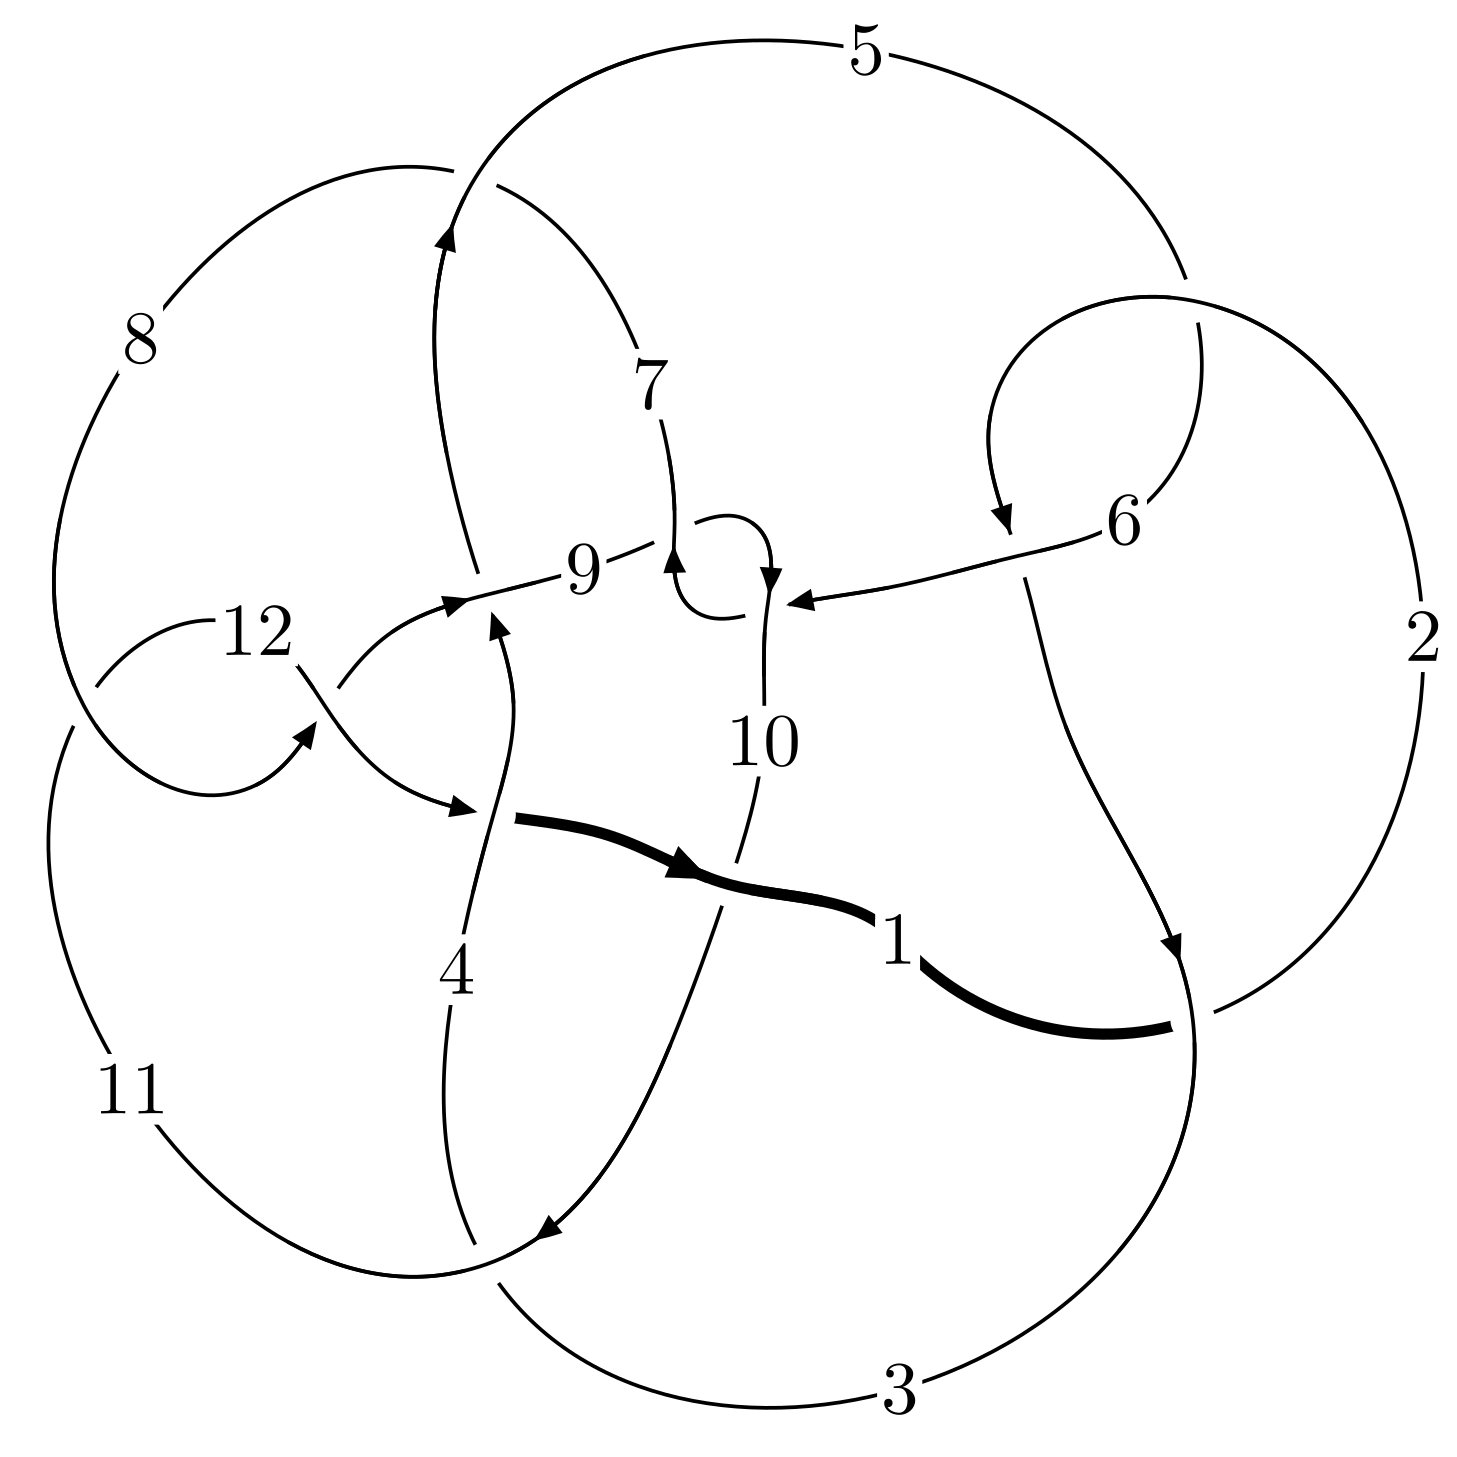
\includegraphics[width=112pt]{../../../GIT/diagram.site/Diagrams/png/1276_12a_0475.png}\\
\ \ \ A knot diagram\footnotemark}&
\allowdisplaybreaks
\textbf{Linearized knot diagam} \\
\cline{2-2}
 &
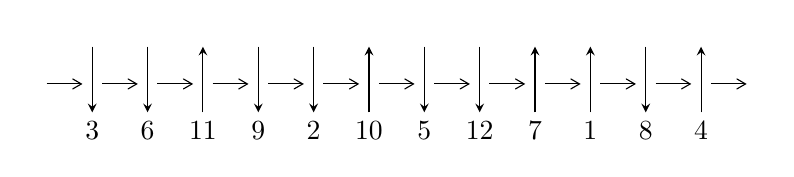
\begin{tikzpicture}[x=20pt, y=17pt]
	% nodes
	\node (C0) at (0, 0) {};
	\node (C1) at (1, 0) {};
	\node (C1U) at (1, +1) {};
	\node (C1D) at (1, -1) {3};

	\node (C2) at (2, 0) {};
	\node (C2U) at (2, +1) {};
	\node (C2D) at (2, -1) {6};

	\node (C3) at (3, 0) {};
	\node (C3U) at (3, +1) {};
	\node (C3D) at (3, -1) {11};

	\node (C4) at (4, 0) {};
	\node (C4U) at (4, +1) {};
	\node (C4D) at (4, -1) {9};

	\node (C5) at (5, 0) {};
	\node (C5U) at (5, +1) {};
	\node (C5D) at (5, -1) {2};

	\node (C6) at (6, 0) {};
	\node (C6U) at (6, +1) {};
	\node (C6D) at (6, -1) {10};

	\node (C7) at (7, 0) {};
	\node (C7U) at (7, +1) {};
	\node (C7D) at (7, -1) {5};

	\node (C8) at (8, 0) {};
	\node (C8U) at (8, +1) {};
	\node (C8D) at (8, -1) {12};

	\node (C9) at (9, 0) {};
	\node (C9U) at (9, +1) {};
	\node (C9D) at (9, -1) {7};

	\node (C10) at (10, 0) {};
	\node (C10U) at (10, +1) {};
	\node (C10D) at (10, -1) {1};

	\node (C11) at (11, 0) {};
	\node (C11U) at (11, +1) {};
	\node (C11D) at (11, -1) {8};

	\node (C12) at (12, 0) {};
	\node (C12U) at (12, +1) {};
	\node (C12D) at (12, -1) {4};
	\node (C13) at (13, 0) {};

	% arrows
	\draw[->,>={angle 60}]
	(C0) edge (C1) (C1) edge (C2) (C2) edge (C3) (C3) edge (C4) (C4) edge (C5) (C5) edge (C6) (C6) edge (C7) (C7) edge (C8) (C8) edge (C9) (C9) edge (C10) (C10) edge (C11) (C11) edge (C12) (C12) edge (C13) ;	\draw[->,>=stealth]
	(C1U) edge (C1D) (C2U) edge (C2D) (C3D) edge (C3U) (C4U) edge (C4D) (C5U) edge (C5D) (C6D) edge (C6U) (C7U) edge (C7D) (C8U) edge (C8D) (C9D) edge (C9U) (C10D) edge (C10U) (C11U) edge (C11D) (C12D) edge (C12U) ;
	\end{tikzpicture} \\
\hhline{~~} \\& 
\textbf{Solving Sequence} \\ \cline{2-2} 
 &
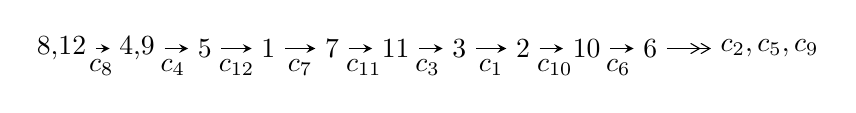
\begin{tikzpicture}[x=23pt, y=7pt]
	% node
	\node (A0) at (-1/8, 0) {8,12};
	\node (A1) at (17/16, 0) {4,9};
	\node (A2) at (17/8, 0) {5};
	\node (A3) at (25/8, 0) {1};
	\node (A4) at (33/8, 0) {7};
	\node (A5) at (41/8, 0) {11};
	\node (A6) at (49/8, 0) {3};
	\node (A7) at (57/8, 0) {2};
	\node (A8) at (65/8, 0) {10};
	\node (A9) at (73/8, 0) {6};
	\node (C1) at (1/2, -1) {$c_{8}$};
	\node (C2) at (13/8, -1) {$c_{4}$};
	\node (C3) at (21/8, -1) {$c_{12}$};
	\node (C4) at (29/8, -1) {$c_{7}$};
	\node (C5) at (37/8, -1) {$c_{11}$};
	\node (C6) at (45/8, -1) {$c_{3}$};
	\node (C7) at (53/8, -1) {$c_{1}$};
	\node (C8) at (61/8, -1) {$c_{10}$};
	\node (C9) at (69/8, -1) {$c_{6}$};
	\node (A10) at (11, 0) {$c_{2},c_{5},c_{9}$};

	% edge
	\draw[->,>=stealth]	
	(A0) edge (A1) (A1) edge (A2) (A2) edge (A3) (A3) edge (A4) (A4) edge (A5) (A5) edge (A6) (A6) edge (A7) (A7) edge (A8) (A8) edge (A9) ;
	\draw[->>,>={angle 60}]	
	(A9) edge (A10);
\end{tikzpicture} \\ 

\end{tabular} \\

\footnotetext{
The image of knot diagram is generated by the software ``\textbf{Draw programme}" developed by Andrew Bartholomew(\url{http://www.layer8.co.uk/maths/draw/index.htm\#Running-draw}), where we modified some parts for our purpose(\url{https://github.com/CATsTAILs/LinksPainter}).
}\phantom \\ \newline 
\centering \textbf{Ideals for irreducible components\footnotemark of $X_{\text{par}}$} 
 
\begin{align*}
I^u_{1}&=\langle 
1.11285\times10^{886} u^{164}-3.44078\times10^{886} u^{163}+\cdots+2.18377\times10^{886} b-6.10321\times10^{889},\\
\phantom{I^u_{1}}&\phantom{= \langle  }2.17789\times10^{889} u^{164}-6.46304\times10^{889} u^{163}+\cdots+5.77716\times10^{889} a-9.99945\times10^{892},\\
\phantom{I^u_{1}}&\phantom{= \langle  }u^{165}-4 u^{164}+\cdots-92466 u+5291\rangle \\
I^u_{2}&=\langle 
1.21748\times10^{26} u^{32}-5.54627\times10^{26} u^{31}+\cdots+2.64218\times10^{26} b+3.56406\times10^{26},\\
\phantom{I^u_{2}}&\phantom{= \langle  }1.91198\times10^{27} u^{32}-8.59389\times10^{27} u^{31}+\cdots+7.92654\times10^{26} a-1.02616\times10^{28},\;u^{33}-4 u^{32}+\cdots+u-3\rangle \\
I^u_{3}&=\langle 
b- a+1,\;a^2-2 a+3,\;u+1\rangle \\
I^u_{4}&=\langle 
2 b-3 a-2,\;a^2+2,\;u+1\rangle \\
I^u_{5}&=\langle 
b,\;a+1,\;u-1\rangle \\
\\
\end{align*}
\raggedright * 5 irreducible components of $\dim_{\mathbb{C}}=0$, with total 203 representations.\\
\footnotetext{All coefficients of polynomials are rational numbers. But the coefficients are sometimes approximated in decimal forms when there is not enough margin.}
\newpage
\renewcommand{\arraystretch}{1}
\centering \section*{I. $I^u_{1}= \langle 1.11\times10^{886} u^{164}-3.44\times10^{886} u^{163}+\cdots+2.18\times10^{886} b-6.10\times10^{889},\;2.18\times10^{889} u^{164}-6.46\times10^{889} u^{163}+\cdots+5.78\times10^{889} a-1.00\times10^{893},\;u^{165}-4 u^{164}+\cdots-92466 u+5291 \rangle$}
\flushleft \textbf{(i) Arc colorings}\\
\begin{tabular}{m{7pt} m{180pt} m{7pt} m{180pt} }
\flushright $a_{8}=$&$\begin{pmatrix}1\\0\end{pmatrix}$ \\
\flushright $a_{12}=$&$\begin{pmatrix}0\\u\end{pmatrix}$ \\
\flushright $a_{4}=$&$\begin{pmatrix}-0.376983 u^{164}+1.11872 u^{163}+\cdots-28825.3 u+1730.86\\-0.509600 u^{164}+1.57562 u^{163}+\cdots-46058.6 u+2794.81\end{pmatrix}$ \\
\flushright $a_{9}=$&$\begin{pmatrix}1\\u^2\end{pmatrix}$ \\
\flushright $a_{5}=$&$\begin{pmatrix}-0.245282 u^{164}+0.714234 u^{163}+\cdots-16760.6 u+995.355\\-0.396999 u^{164}+1.22308 u^{163}+\cdots-35445.4 u+2147.63\end{pmatrix}$ \\
\flushright $a_{1}=$&$\begin{pmatrix}-0.437933 u^{164}+1.40631 u^{163}+\cdots-42794.0 u+2610.44\\-0.302392 u^{164}+0.991408 u^{163}+\cdots-31579.1 u+1932.62\end{pmatrix}$ \\
\flushright $a_{7}=$&$\begin{pmatrix}0.196129 u^{164}-0.649218 u^{163}+\cdots+22352.2 u-1359.29\\0.145758 u^{164}-0.521515 u^{163}+\cdots+20402.8 u-1262.91\end{pmatrix}$ \\
\flushright $a_{11}=$&$\begin{pmatrix}u\\u\end{pmatrix}$ \\
\flushright $a_{3}=$&$\begin{pmatrix}-0.349509 u^{164}+0.998201 u^{163}+\cdots-22723.8 u+1341.57\\-0.482126 u^{164}+1.45509 u^{163}+\cdots-39957.1 u+2405.52\end{pmatrix}$ \\
\flushright $a_{2}=$&$\begin{pmatrix}-0.0587150 u^{164}+0.149057 u^{163}+\cdots-794.726 u+25.6789\\-0.0254560 u^{164}+0.118769 u^{163}+\cdots-5333.39 u+339.046\end{pmatrix}$ \\
\flushright $a_{10}=$&$\begin{pmatrix}0.0812809 u^{164}-0.202180 u^{163}+\cdots+1666.04 u-68.9146\\0.180251 u^{164}-0.493538 u^{163}+\cdots+10195.9 u-586.870\end{pmatrix}$ \\
\flushright $a_{6}=$&$\begin{pmatrix}-0.0206187 u^{164}+0.0815913 u^{163}+\cdots-4604.61 u+297.410\\-0.159919 u^{164}+0.467206 u^{163}+\cdots-12375.5 u+739.339\end{pmatrix}$\\&\end{tabular}
\flushleft \textbf{(ii) Obstruction class $= -1$}\\~\\
\flushleft \textbf{(iii) Cusp Shapes $= 0.660587 u^{164}-1.95887 u^{163}+\cdots+50154.9 u-3011.11$}\\~\\
\newpage\renewcommand{\arraystretch}{1}
\flushleft \textbf{(iv) u-Polynomials at the component}\newline \\
\begin{tabular}{m{50pt}|m{274pt}}
Crossings & \hspace{64pt}u-Polynomials at each crossing \\
\hline $$\begin{aligned}c_{1}\end{aligned}$$&$\begin{aligned}
&u^{165}+73 u^{164}+\cdots+5492581 u+346921
\end{aligned}$\\
\hline $$\begin{aligned}c_{2},c_{5}\end{aligned}$$&$\begin{aligned}
&u^{165}+5 u^{164}+\cdots-2107 u+589
\end{aligned}$\\
\hline $$\begin{aligned}c_{3}\end{aligned}$$&$\begin{aligned}
&2(2 u^{165}-6 u^{164}+\cdots-6475 u+1861)
\end{aligned}$\\
\hline $$\begin{aligned}c_{4}\end{aligned}$$&$\begin{aligned}
&2(2 u^{165}+4 u^{164}+\cdots-1.28570\times10^{8} u-1.40072\times10^{8})
\end{aligned}$\\
\hline $$\begin{aligned}c_{6},c_{9}\end{aligned}$$&$\begin{aligned}
&u^{165}+11 u^{164}+\cdots+593536 u+54052
\end{aligned}$\\
\hline $$\begin{aligned}c_{7}\end{aligned}$$&$\begin{aligned}
&u^{165}-11 u^{164}+\cdots-13275136 u+1499648
\end{aligned}$\\
\hline $$\begin{aligned}c_{8},c_{11}\end{aligned}$$&$\begin{aligned}
&u^{165}+4 u^{164}+\cdots-92466 u-5291
\end{aligned}$\\
\hline $$\begin{aligned}c_{10}\end{aligned}$$&$\begin{aligned}
&u^{165}+18 u^{164}+\cdots-1283584 u-111872
\end{aligned}$\\
\hline $$\begin{aligned}c_{12}\end{aligned}$$&$\begin{aligned}
&u^{165}+16 u^{164}+\cdots+1428492 u+35066
\end{aligned}$\\
\hline
\end{tabular}\\~\\
\newpage\renewcommand{\arraystretch}{1}
\flushleft \textbf{(v) Riley Polynomials at the component}\newline \\
\begin{tabular}{m{50pt}|m{274pt}}
Crossings & \hspace{64pt}Riley Polynomials at each crossing \\
\hline $$\begin{aligned}c_{1}\end{aligned}$$&$\begin{aligned}
&y^{165}+47 y^{164}+\cdots+929433493849 y-120354180241
\end{aligned}$\\
\hline $$\begin{aligned}c_{2},c_{5}\end{aligned}$$&$\begin{aligned}
&y^{165}-73 y^{164}+\cdots+5492581 y-346921
\end{aligned}$\\
\hline $$\begin{aligned}c_{3}\end{aligned}$$&$\begin{aligned}
&4(4 y^{165}-120 y^{164}+\cdots+2.97286\times10^{7} y-3463321)
\end{aligned}$\\
\hline $$\begin{aligned}c_{4}\end{aligned}$$&$\begin{aligned}
&4(4 y^{165}-228 y^{164}+\cdots+1.18967\times10^{18} y-1.96202\times10^{16})
\end{aligned}$\\
\hline $$\begin{aligned}c_{6},c_{9}\end{aligned}$$&$\begin{aligned}
&y^{165}+125 y^{164}+\cdots+44245013584 y-2921618704
\end{aligned}$\\
\hline $$\begin{aligned}c_{7}\end{aligned}$$&$\begin{aligned}
&y^{165}-25 y^{164}+\cdots+95755580735488 y-2248944123904
\end{aligned}$\\
\hline $$\begin{aligned}c_{8},c_{11}\end{aligned}$$&$\begin{aligned}
&y^{165}-98 y^{164}+\cdots+2317734584 y-27994681
\end{aligned}$\\
\hline $$\begin{aligned}c_{10}\end{aligned}$$&$\begin{aligned}
&y^{165}+16 y^{164}+\cdots-906086514688 y-12515344384
\end{aligned}$\\
\hline $$\begin{aligned}c_{12}\end{aligned}$$&$\begin{aligned}
&y^{165}+50 y^{164}+\cdots+436180962572 y-1229624356
\end{aligned}$\\
\hline
\end{tabular}\\~\\
\newpage\flushleft \textbf{(vi) Complex Volumes and Cusp Shapes}
$$\begin{array}{c|c|c}  
\text{Solutions to }I^u_{1}& \I (\text{vol} + \sqrt{-1}CS) & \text{Cusp shape}\\
 \hline 
\begin{aligned}
u &= -0.905625 + 0.395022 I \\
a &= -1.356160 - 0.178801 I \\
b &= -0.500288 + 0.541412 I\end{aligned}
 & \phantom{-}1.76132 + 6.82155 I & \phantom{-0.000000 } 0 \\ \hline\begin{aligned}
u &= -0.905625 - 0.395022 I \\
a &= -1.356160 + 0.178801 I \\
b &= -0.500288 - 0.541412 I\end{aligned}
 & \phantom{-}1.76132 - 6.82155 I & \phantom{-0.000000 } 0 \\ \hline\begin{aligned}
u &= \phantom{-}0.979945 + 0.253064 I \\
a &= \phantom{-}2.14093 - 0.15484 I \\
b &= \phantom{-}1.245890 + 0.373436 I\end{aligned}
 & -2.68322 - 10.66630 I & \phantom{-0.000000 } 0 \\ \hline\begin{aligned}
u &= \phantom{-}0.979945 - 0.253064 I \\
a &= \phantom{-}2.14093 + 0.15484 I \\
b &= \phantom{-}1.245890 - 0.373436 I\end{aligned}
 & -2.68322 + 10.66630 I & \phantom{-0.000000 } 0 \\ \hline\begin{aligned}
u &= -1.010130 + 0.104708 I \\
a &= \phantom{-}0.66284 - 1.49523 I \\
b &= -0.67789 - 2.01547 I\end{aligned}
 & -7.16497 + 2.22800 I & \phantom{-0.000000 } 0 \\ \hline\begin{aligned}
u &= -1.010130 - 0.104708 I \\
a &= \phantom{-}0.66284 + 1.49523 I \\
b &= -0.67789 + 2.01547 I\end{aligned}
 & -7.16497 - 2.22800 I & \phantom{-0.000000 } 0 \\ \hline\begin{aligned}
u &= -0.911483 + 0.450030 I \\
a &= \phantom{-}0.43769 - 1.68406 I \\
b &= \phantom{-}0.43601 - 1.82372 I\end{aligned}
 & -4.66672 - 1.50795 I & \phantom{-0.000000 } 0 \\ \hline\begin{aligned}
u &= -0.911483 - 0.450030 I \\
a &= \phantom{-}0.43769 + 1.68406 I \\
b &= \phantom{-}0.43601 + 1.82372 I\end{aligned}
 & -4.66672 + 1.50795 I & \phantom{-0.000000 } 0 \\ \hline\begin{aligned}
u &= \phantom{-}0.949136 + 0.247064 I \\
a &= -1.98722 + 0.29565 I \\
b &= -0.987252 - 0.036458 I\end{aligned}
 & -0.24597 - 4.87496 I & \phantom{-0.000000 } 0 \\ \hline\begin{aligned}
u &= \phantom{-}0.949136 - 0.247064 I \\
a &= -1.98722 - 0.29565 I \\
b &= -0.987252 + 0.036458 I\end{aligned}
 & -0.24597 + 4.87496 I & \phantom{-0.000000 } 0\\
 \hline 
 \end{array}$$\newpage$$\begin{array}{c|c|c}  
\text{Solutions to }I^u_{1}& \I (\text{vol} + \sqrt{-1}CS) & \text{Cusp shape}\\
 \hline 
\begin{aligned}
u &= -0.956326 + 0.354024 I \\
a &= \phantom{-}0.472835 + 0.991788 I \\
b &= \phantom{-}0.96915 + 2.16384 I\end{aligned}
 & \phantom{-}0.39699 + 5.70050 I & \phantom{-0.000000 } 0 \\ \hline\begin{aligned}
u &= -0.956326 - 0.354024 I \\
a &= \phantom{-}0.472835 - 0.991788 I \\
b &= \phantom{-}0.96915 - 2.16384 I\end{aligned}
 & \phantom{-}0.39699 - 5.70050 I & \phantom{-0.000000 } 0 \\ \hline\begin{aligned}
u &= \phantom{-}0.997397 + 0.222897 I \\
a &= \phantom{-}0.045810 - 0.837141 I \\
b &= \phantom{-}1.30671 - 2.18702 I\end{aligned}
 & \phantom{-}0.02937 - 6.00270 I & \phantom{-0.000000 } 0 \\ \hline\begin{aligned}
u &= \phantom{-}0.997397 - 0.222897 I \\
a &= \phantom{-}0.045810 + 0.837141 I \\
b &= \phantom{-}1.30671 + 2.18702 I\end{aligned}
 & \phantom{-}0.02937 + 6.00270 I & \phantom{-0.000000 } 0 \\ \hline\begin{aligned}
u &= \phantom{-}1.029100 + 0.039524 I \\
a &= -0.152827 - 0.504647 I \\
b &= \phantom{-}1.17849 - 2.45752 I\end{aligned}
 & -3.31303 + 0.23435 I & \phantom{-0.000000 } 0 \\ \hline\begin{aligned}
u &= \phantom{-}1.029100 - 0.039524 I \\
a &= -0.152827 + 0.504647 I \\
b &= \phantom{-}1.17849 + 2.45752 I\end{aligned}
 & -3.31303 - 0.23435 I & \phantom{-0.000000 } 0 \\ \hline\begin{aligned}
u &= \phantom{-}0.056114 + 0.961060 I \\
a &= \phantom{-}0.004362 + 0.793680 I \\
b &= \phantom{-}0.522822 - 0.084660 I\end{aligned}
 & \phantom{-}0.53874 - 4.38609 I & \phantom{-0.000000 } 0 \\ \hline\begin{aligned}
u &= \phantom{-}0.056114 - 0.961060 I \\
a &= \phantom{-}0.004362 - 0.793680 I \\
b &= \phantom{-}0.522822 + 0.084660 I\end{aligned}
 & \phantom{-}0.53874 + 4.38609 I & \phantom{-0.000000 } 0 \\ \hline\begin{aligned}
u &= \phantom{-}0.265842 + 0.916273 I \\
a &= \phantom{-}0.090527 + 0.910352 I \\
b &= \phantom{-}0.219918 - 0.118177 I\end{aligned}
 & \phantom{-}0.1210590 - 0.0627933 I & \phantom{-0.000000 } 0 \\ \hline\begin{aligned}
u &= \phantom{-}0.265842 - 0.916273 I \\
a &= \phantom{-}0.090527 - 0.910352 I \\
b &= \phantom{-}0.219918 + 0.118177 I\end{aligned}
 & \phantom{-}0.1210590 + 0.0627933 I & \phantom{-0.000000 } 0\\
 \hline 
 \end{array}$$\newpage$$\begin{array}{c|c|c}  
\text{Solutions to }I^u_{1}& \I (\text{vol} + \sqrt{-1}CS) & \text{Cusp shape}\\
 \hline 
\begin{aligned}
u &= \phantom{-}0.928790 + 0.214195 I \\
a &= -0.166509 + 0.819530 I \\
b &= -1.24767 + 2.01704 I\end{aligned}
 & \phantom{-}1.59672 - 0.72836 I & \phantom{-0.000000 } 0 \\ \hline\begin{aligned}
u &= \phantom{-}0.928790 - 0.214195 I \\
a &= -0.166509 - 0.819530 I \\
b &= -1.24767 - 2.01704 I\end{aligned}
 & \phantom{-}1.59672 + 0.72836 I & \phantom{-0.000000 } 0 \\ \hline\begin{aligned}
u &= \phantom{-}0.208224 + 0.928754 I \\
a &= -0.939974 - 0.108861 I \\
b &= \phantom{-}0.032619 - 0.688229 I\end{aligned}
 & -1.44989 - 2.06089 I & \phantom{-0.000000 } 0 \\ \hline\begin{aligned}
u &= \phantom{-}0.208224 - 0.928754 I \\
a &= -0.939974 + 0.108861 I \\
b &= \phantom{-}0.032619 + 0.688229 I\end{aligned}
 & -1.44989 + 2.06089 I & \phantom{-0.000000 } 0 \\ \hline\begin{aligned}
u &= \phantom{-}0.099343 + 0.945992 I \\
a &= \phantom{-}1.211790 - 0.585575 I \\
b &= \phantom{-}0.159309 + 0.050813 I\end{aligned}
 & -7.38673 + 5.98012 I & \phantom{-0.000000 } 0 \\ \hline\begin{aligned}
u &= \phantom{-}0.099343 - 0.945992 I \\
a &= \phantom{-}1.211790 + 0.585575 I \\
b &= \phantom{-}0.159309 - 0.050813 I\end{aligned}
 & -7.38673 - 5.98012 I & \phantom{-0.000000 } 0 \\ \hline\begin{aligned}
u &= -1.004120 + 0.343761 I \\
a &= -0.415362 - 0.862654 I \\
b &= -1.09118 - 2.32631 I\end{aligned}
 & -2.25182 + 11.57660 I & \phantom{-0.000000 } 0 \\ \hline\begin{aligned}
u &= -1.004120 - 0.343761 I \\
a &= -0.415362 + 0.862654 I \\
b &= -1.09118 + 2.32631 I\end{aligned}
 & -2.25182 - 11.57660 I & \phantom{-0.000000 } 0 \\ \hline\begin{aligned}
u &= -0.543395 + 0.919447 I \\
a &= -0.227727 + 0.555914 I \\
b &= -0.439377 - 0.320989 I\end{aligned}
 & \phantom{-}0.479910 + 0.205738 I & \phantom{-0.000000 } 0 \\ \hline\begin{aligned}
u &= -0.543395 - 0.919447 I \\
a &= -0.227727 - 0.555914 I \\
b &= -0.439377 + 0.320989 I\end{aligned}
 & \phantom{-}0.479910 - 0.205738 I & \phantom{-0.000000 } 0\\
 \hline 
 \end{array}$$\newpage$$\begin{array}{c|c|c}  
\text{Solutions to }I^u_{1}& \I (\text{vol} + \sqrt{-1}CS) & \text{Cusp shape}\\
 \hline 
\begin{aligned}
u &= -0.921973 + 0.064761 I \\
a &= -0.58718 + 1.64883 I \\
b &= \phantom{-}0.75741 + 1.83648 I\end{aligned}
 & -6.76898 - 1.45593 I & \phantom{-0.000000 } 0 \\ \hline\begin{aligned}
u &= -0.921973 - 0.064761 I \\
a &= -0.58718 - 1.64883 I \\
b &= \phantom{-}0.75741 - 1.83648 I\end{aligned}
 & -6.76898 + 1.45593 I & \phantom{-0.000000 } 0 \\ \hline\begin{aligned}
u &= \phantom{-}0.058757 + 1.081710 I \\
a &= -0.661431 - 0.299147 I \\
b &= \phantom{-}0.126078 - 0.124589 I\end{aligned}
 & -0.89907 - 2.39252 I & \phantom{-0.000000 } 0 \\ \hline\begin{aligned}
u &= \phantom{-}0.058757 - 1.081710 I \\
a &= -0.661431 + 0.299147 I \\
b &= \phantom{-}0.126078 + 0.124589 I\end{aligned}
 & -0.89907 + 2.39252 I & \phantom{-0.000000 } 0 \\ \hline\begin{aligned}
u &= \phantom{-}0.879166 + 0.214573 I \\
a &= \phantom{-}2.19850 - 1.13943 I \\
b &= \phantom{-}1.69238 - 1.06824 I\end{aligned}
 & -6.36992 - 1.10734 I & \phantom{-0.000000 } 0 \\ \hline\begin{aligned}
u &= \phantom{-}0.879166 - 0.214573 I \\
a &= \phantom{-}2.19850 + 1.13943 I \\
b &= \phantom{-}1.69238 + 1.06824 I\end{aligned}
 & -6.36992 + 1.10734 I & \phantom{-0.000000 } 0 \\ \hline\begin{aligned}
u &= \phantom{-}1.057980 + 0.337150 I \\
a &= \phantom{-}0.94946 - 1.39230 I \\
b &= \phantom{-}0.50194 - 2.07114 I\end{aligned}
 & -6.46535 - 0.46060 I & \phantom{-0.000000 } 0 \\ \hline\begin{aligned}
u &= \phantom{-}1.057980 - 0.337150 I \\
a &= \phantom{-}0.94946 + 1.39230 I \\
b &= \phantom{-}0.50194 + 2.07114 I\end{aligned}
 & -6.46535 + 0.46060 I & \phantom{-0.000000 } 0 \\ \hline\begin{aligned}
u &= \phantom{-}0.458763 + 1.011900 I \\
a &= \phantom{-}0.901403 + 0.412848 I \\
b &= -0.384411 + 0.936939 I\end{aligned}
 & -3.08963 - 6.66268 I & \phantom{-0.000000 } 0 \\ \hline\begin{aligned}
u &= \phantom{-}0.458763 - 1.011900 I \\
a &= \phantom{-}0.901403 - 0.412848 I \\
b &= -0.384411 - 0.936939 I\end{aligned}
 & -3.08963 + 6.66268 I & \phantom{-0.000000 } 0\\
 \hline 
 \end{array}$$\newpage$$\begin{array}{c|c|c}  
\text{Solutions to }I^u_{1}& \I (\text{vol} + \sqrt{-1}CS) & \text{Cusp shape}\\
 \hline 
\begin{aligned}
u &= -0.830270 + 0.293600 I \\
a &= -1.142810 - 0.693487 I \\
b &= -0.47384 - 1.88262 I\end{aligned}
 & -5.83699 + 1.41896 I & \phantom{-0.000000 } 0 \\ \hline\begin{aligned}
u &= -0.830270 - 0.293600 I \\
a &= -1.142810 + 0.693487 I \\
b &= -0.47384 + 1.88262 I\end{aligned}
 & -5.83699 - 1.41896 I & \phantom{-0.000000 } 0 \\ \hline\begin{aligned}
u &= -1.092040 + 0.250124 I \\
a &= -0.53036 - 1.35874 I \\
b &= -0.65812 - 2.06798 I\end{aligned}
 & -4.49963 + 0.97465 I & \phantom{-0.000000 } 0 \\ \hline\begin{aligned}
u &= -1.092040 - 0.250124 I \\
a &= -0.53036 + 1.35874 I \\
b &= -0.65812 + 2.06798 I\end{aligned}
 & -4.49963 - 0.97465 I & \phantom{-0.000000 } 0 \\ \hline\begin{aligned}
u &= \phantom{-}1.112570 + 0.146778 I \\
a &= \phantom{-}0.086327 + 0.326728 I \\
b &= -0.72273 + 1.56197 I\end{aligned}
 & -3.30358 + 0.53754 I & \phantom{-0.000000 } 0 \\ \hline\begin{aligned}
u &= \phantom{-}1.112570 - 0.146778 I \\
a &= \phantom{-}0.086327 - 0.326728 I \\
b &= -0.72273 - 1.56197 I\end{aligned}
 & -3.30358 - 0.53754 I & \phantom{-0.000000 } 0 \\ \hline\begin{aligned}
u &= -0.790955 + 0.377288 I \\
a &= \phantom{-}1.51363 + 0.25917 I \\
b &= \phantom{-}0.477732 - 0.416986 I\end{aligned}
 & \phantom{-}3.18590 + 1.28226 I & \phantom{-0.000000 } 0 \\ \hline\begin{aligned}
u &= -0.790955 - 0.377288 I \\
a &= \phantom{-}1.51363 - 0.25917 I \\
b &= \phantom{-}0.477732 + 0.416986 I\end{aligned}
 & \phantom{-}3.18590 - 1.28226 I & \phantom{-0.000000 } 0 \\ \hline\begin{aligned}
u &= \phantom{-}0.751764 + 0.835486 I \\
a &= \phantom{-}0.106249 - 0.125011 I \\
b &= \phantom{-}0.452743 - 0.287726 I\end{aligned}
 & -0.70273 - 1.40924 I & \phantom{-0.000000 } 0 \\ \hline\begin{aligned}
u &= \phantom{-}0.751764 - 0.835486 I \\
a &= \phantom{-}0.106249 + 0.125011 I \\
b &= \phantom{-}0.452743 + 0.287726 I\end{aligned}
 & -0.70273 + 1.40924 I & \phantom{-0.000000 } 0\\
 \hline 
 \end{array}$$\newpage$$\begin{array}{c|c|c}  
\text{Solutions to }I^u_{1}& \I (\text{vol} + \sqrt{-1}CS) & \text{Cusp shape}\\
 \hline 
\begin{aligned}
u &= \phantom{-}0.228998 + 1.105140 I \\
a &= -1.029760 + 0.398436 I \\
b &= -0.127356 - 0.341013 I\end{aligned}
 & -0.69256 + 8.20346 I & \phantom{-0.000000 } 0 \\ \hline\begin{aligned}
u &= \phantom{-}0.228998 - 1.105140 I \\
a &= -1.029760 - 0.398436 I \\
b &= -0.127356 + 0.341013 I\end{aligned}
 & -0.69256 - 8.20346 I & \phantom{-0.000000 } 0 \\ \hline\begin{aligned}
u &= -0.867320\phantom{ +0.000000I} \\
a &= -1.90161\phantom{ +0.000000I} \\
b &= -1.09360\phantom{ +0.000000I}\end{aligned}
 & -2.84073\phantom{ +0.000000I} & \phantom{-0.000000 } 0 \\ \hline\begin{aligned}
u &= \phantom{-}0.406558 + 0.763432 I \\
a &= -0.057417 - 1.060420 I \\
b &= -0.1342720 - 0.0332840 I\end{aligned}
 & \phantom{-}0.00310 - 4.02060 I & \phantom{-0.000000 } 0 \\ \hline\begin{aligned}
u &= \phantom{-}0.406558 - 0.763432 I \\
a &= -0.057417 + 1.060420 I \\
b &= -0.1342720 + 0.0332840 I\end{aligned}
 & \phantom{-}0.00310 + 4.02060 I & \phantom{-0.000000 } 0 \\ \hline\begin{aligned}
u &= -0.975283 + 0.581760 I \\
a &= -1.09940 + 1.14684 I \\
b &= -0.99216 + 1.59918 I\end{aligned}
 & -5.06065 + 5.72523 I & \phantom{-0.000000 } 0 \\ \hline\begin{aligned}
u &= -0.975283 - 0.581760 I \\
a &= -1.09940 - 1.14684 I \\
b &= -0.99216 - 1.59918 I\end{aligned}
 & -5.06065 - 5.72523 I & \phantom{-0.000000 } 0 \\ \hline\begin{aligned}
u &= -1.135730 + 0.035452 I \\
a &= \phantom{-}0.609597 - 1.261730 I \\
b &= -0.29117 - 2.00297 I\end{aligned}
 & -6.86660 - 2.87605 I & \phantom{-0.000000 } 0 \\ \hline\begin{aligned}
u &= -1.135730 - 0.035452 I \\
a &= \phantom{-}0.609597 + 1.261730 I \\
b &= -0.29117 + 2.00297 I\end{aligned}
 & -6.86660 + 2.87605 I & \phantom{-0.000000 } 0 \\ \hline\begin{aligned}
u &= -0.024095 + 0.861263 I \\
a &= \phantom{-}0.069793 - 0.747455 I \\
b &= -0.602458 - 0.116725 I\end{aligned}
 & \phantom{-}0.940791 - 0.237333 I & \phantom{-0.000000 } 0\\
 \hline 
 \end{array}$$\newpage$$\begin{array}{c|c|c}  
\text{Solutions to }I^u_{1}& \I (\text{vol} + \sqrt{-1}CS) & \text{Cusp shape}\\
 \hline 
\begin{aligned}
u &= -0.024095 - 0.861263 I \\
a &= \phantom{-}0.069793 + 0.747455 I \\
b &= -0.602458 + 0.116725 I\end{aligned}
 & \phantom{-}0.940791 + 0.237333 I & \phantom{-0.000000 } 0 \\ \hline\begin{aligned}
u &= -0.298727 + 1.120920 I \\
a &= \phantom{-}0.850074 + 0.284549 I \\
b &= -0.098946 - 0.430575 I\end{aligned}
 & \phantom{-}3.31062 - 2.35546 I & \phantom{-0.000000 } 0 \\ \hline\begin{aligned}
u &= -0.298727 - 1.120920 I \\
a &= \phantom{-}0.850074 - 0.284549 I \\
b &= -0.098946 + 0.430575 I\end{aligned}
 & \phantom{-}3.31062 + 2.35546 I & \phantom{-0.000000 } 0 \\ \hline\begin{aligned}
u &= -0.804266 + 0.838329 I \\
a &= \phantom{-}0.014358 - 0.556604 I \\
b &= \phantom{-}0.483803 + 0.156529 I\end{aligned}
 & -0.26591 + 6.01439 I & \phantom{-0.000000 } 0 \\ \hline\begin{aligned}
u &= -0.804266 - 0.838329 I \\
a &= \phantom{-}0.014358 + 0.556604 I \\
b &= \phantom{-}0.483803 - 0.156529 I\end{aligned}
 & -0.26591 - 6.01439 I & \phantom{-0.000000 } 0 \\ \hline\begin{aligned}
u &= -1.160280 + 0.071947 I \\
a &= -0.382685 - 1.121420 I \\
b &= \phantom{-}0.30068 - 1.66006 I\end{aligned}
 & -5.77557 - 1.21497 I & \phantom{-0.000000 } 0 \\ \hline\begin{aligned}
u &= -1.160280 - 0.071947 I \\
a &= -0.382685 + 1.121420 I \\
b &= \phantom{-}0.30068 + 1.66006 I\end{aligned}
 & -5.77557 + 1.21497 I & \phantom{-0.000000 } 0 \\ \hline\begin{aligned}
u &= \phantom{-}0.993491 + 0.613036 I \\
a &= -0.053013 + 0.207665 I \\
b &= -0.676586 + 0.767305 I\end{aligned}
 & -1.88344 - 5.23161 I & \phantom{-0.000000 } 0 \\ \hline\begin{aligned}
u &= \phantom{-}0.993491 - 0.613036 I \\
a &= -0.053013 - 0.207665 I \\
b &= -0.676586 - 0.767305 I\end{aligned}
 & -1.88344 + 5.23161 I & \phantom{-0.000000 } 0 \\ \hline\begin{aligned}
u &= \phantom{-}0.806218 + 0.186328 I \\
a &= -1.48357 - 0.17893 I \\
b &= \phantom{-}0.316977 - 0.132627 I\end{aligned}
 & \phantom{-}2.03513 - 1.28246 I & \phantom{-0.000000 } 0\\
 \hline 
 \end{array}$$\newpage$$\begin{array}{c|c|c}  
\text{Solutions to }I^u_{1}& \I (\text{vol} + \sqrt{-1}CS) & \text{Cusp shape}\\
 \hline 
\begin{aligned}
u &= \phantom{-}0.806218 - 0.186328 I \\
a &= -1.48357 + 0.17893 I \\
b &= \phantom{-}0.316977 + 0.132627 I\end{aligned}
 & \phantom{-}2.03513 + 1.28246 I & \phantom{-0.000000 } 0 \\ \hline\begin{aligned}
u &= \phantom{-}0.181258 + 1.161330 I \\
a &= \phantom{-}0.966257 - 0.450421 I \\
b &= \phantom{-}0.026849 + 0.353142 I\end{aligned}
 & -2.5882 + 14.0878 I & \phantom{-0.000000 } 0 \\ \hline\begin{aligned}
u &= \phantom{-}0.181258 - 1.161330 I \\
a &= \phantom{-}0.966257 + 0.450421 I \\
b &= \phantom{-}0.026849 - 0.353142 I\end{aligned}
 & -2.5882 - 14.0878 I & \phantom{-0.000000 } 0 \\ \hline\begin{aligned}
u &= -0.700839 + 0.404790 I \\
a &= \phantom{-}0.054640 + 1.215590 I \\
b &= \phantom{-}0.83768 + 1.41021 I\end{aligned}
 & \phantom{-}3.40890 + 2.17216 I & \phantom{-0.000000 } 0 \\ \hline\begin{aligned}
u &= -0.700839 - 0.404790 I \\
a &= \phantom{-}0.054640 - 1.215590 I \\
b &= \phantom{-}0.83768 - 1.41021 I\end{aligned}
 & \phantom{-}3.40890 - 2.17216 I & \phantom{-0.000000 } 0 \\ \hline\begin{aligned}
u &= \phantom{-}1.179340 + 0.215040 I \\
a &= \phantom{-}0.46961 - 1.83928 I \\
b &= \phantom{-}0.95078 - 2.41449 I\end{aligned}
 & -9.46194 - 1.63399 I & \phantom{-0.000000 } 0 \\ \hline\begin{aligned}
u &= \phantom{-}1.179340 - 0.215040 I \\
a &= \phantom{-}0.46961 + 1.83928 I \\
b &= \phantom{-}0.95078 + 2.41449 I\end{aligned}
 & -9.46194 + 1.63399 I & \phantom{-0.000000 } 0 \\ \hline\begin{aligned}
u &= \phantom{-}0.378157 + 0.688670 I \\
a &= -1.64772 + 0.16779 I \\
b &= -0.746451 - 0.075755 I\end{aligned}
 & -1.10643 + 3.08168 I & \phantom{-0.000000 } 0 \\ \hline\begin{aligned}
u &= \phantom{-}0.378157 - 0.688670 I \\
a &= -1.64772 - 0.16779 I \\
b &= -0.746451 + 0.075755 I\end{aligned}
 & -1.10643 - 3.08168 I & \phantom{-0.000000 } 0 \\ \hline\begin{aligned}
u &= \phantom{-}1.093150 + 0.546626 I \\
a &= -0.12095 + 1.69603 I \\
b &= -0.23509 + 2.34390 I\end{aligned}
 & -3.19196 - 7.84564 I & \phantom{-0.000000 } 0\\
 \hline 
 \end{array}$$\newpage$$\begin{array}{c|c|c}  
\text{Solutions to }I^u_{1}& \I (\text{vol} + \sqrt{-1}CS) & \text{Cusp shape}\\
 \hline 
\begin{aligned}
u &= \phantom{-}1.093150 - 0.546626 I \\
a &= -0.12095 - 1.69603 I \\
b &= -0.23509 - 2.34390 I\end{aligned}
 & -3.19196 + 7.84564 I & \phantom{-0.000000 } 0 \\ \hline\begin{aligned}
u &= -1.128490 + 0.473924 I \\
a &= \phantom{-}0.262969 + 1.304190 I \\
b &= \phantom{-}0.61424 + 2.02554 I\end{aligned}
 & -1.21383 + 5.54894 I & \phantom{-0.000000 } 0 \\ \hline\begin{aligned}
u &= -1.128490 - 0.473924 I \\
a &= \phantom{-}0.262969 - 1.304190 I \\
b &= \phantom{-}0.61424 - 2.02554 I\end{aligned}
 & -1.21383 - 5.54894 I & \phantom{-0.000000 } 0 \\ \hline\begin{aligned}
u &= -1.187050 + 0.303700 I \\
a &= \phantom{-}0.166697 + 0.629003 I \\
b &= -1.19563 + 1.36882 I\end{aligned}
 & -9.82340 + 2.80556 I & \phantom{-0.000000 } 0 \\ \hline\begin{aligned}
u &= -1.187050 - 0.303700 I \\
a &= \phantom{-}0.166697 - 0.629003 I \\
b &= -1.19563 - 1.36882 I\end{aligned}
 & -9.82340 - 2.80556 I & \phantom{-0.000000 } 0 \\ \hline\begin{aligned}
u &= \phantom{-}1.206120 + 0.279453 I \\
a &= \phantom{-}0.129864 - 0.613403 I \\
b &= -0.48678 - 1.33134 I\end{aligned}
 & -2.67844 - 1.25468 I & \phantom{-0.000000 } 0 \\ \hline\begin{aligned}
u &= \phantom{-}1.206120 - 0.279453 I \\
a &= \phantom{-}0.129864 + 0.613403 I \\
b &= -0.48678 + 1.33134 I\end{aligned}
 & -2.67844 + 1.25468 I & \phantom{-0.000000 } 0 \\ \hline\begin{aligned}
u &= -0.235723 + 1.225790 I \\
a &= -0.788767 - 0.267827 I \\
b &= \phantom{-}0.275627 + 0.396488 I\end{aligned}
 & \phantom{-}2.18155 - 7.39945 I & \phantom{-0.000000 } 0 \\ \hline\begin{aligned}
u &= -0.235723 - 1.225790 I \\
a &= -0.788767 + 0.267827 I \\
b &= \phantom{-}0.275627 - 0.396488 I\end{aligned}
 & \phantom{-}2.18155 + 7.39945 I & \phantom{-0.000000 } 0 \\ \hline\begin{aligned}
u &= \phantom{-}0.693656 + 0.262829 I \\
a &= -0.90550 + 1.22346 I \\
b &= -1.41372 + 1.35496 I\end{aligned}
 & \phantom{-}0.48947 + 2.43883 I & \phantom{-0.000000 } 0\\
 \hline 
 \end{array}$$\newpage$$\begin{array}{c|c|c}  
\text{Solutions to }I^u_{1}& \I (\text{vol} + \sqrt{-1}CS) & \text{Cusp shape}\\
 \hline 
\begin{aligned}
u &= \phantom{-}0.693656 - 0.262829 I \\
a &= -0.90550 - 1.22346 I \\
b &= -1.41372 - 1.35496 I\end{aligned}
 & \phantom{-}0.48947 - 2.43883 I & \phantom{-0.000000 } 0 \\ \hline\begin{aligned}
u &= -0.544656 + 0.493674 I \\
a &= \phantom{-}0.097345 - 1.142150 I \\
b &= -0.851814 - 1.055840 I\end{aligned}
 & \phantom{-}2.71700 - 3.14847 I & \phantom{-0.000000 } 0 \\ \hline\begin{aligned}
u &= -0.544656 - 0.493674 I \\
a &= \phantom{-}0.097345 + 1.142150 I \\
b &= -0.851814 + 1.055840 I\end{aligned}
 & \phantom{-}2.71700 + 3.14847 I & \phantom{-0.000000 } 0 \\ \hline\begin{aligned}
u &= \phantom{-}0.524400 + 0.509061 I \\
a &= \phantom{-}0.0780599 - 0.0652838 I \\
b &= -0.037059 - 0.599061 I\end{aligned}
 & -0.34407 - 1.50763 I & \phantom{-0.000000 } 0 \\ \hline\begin{aligned}
u &= \phantom{-}0.524400 - 0.509061 I \\
a &= \phantom{-}0.0780599 + 0.0652838 I \\
b &= -0.037059 + 0.599061 I\end{aligned}
 & -0.34407 + 1.50763 I & \phantom{-0.000000 } 0 \\ \hline\begin{aligned}
u &= -0.568060 + 0.445141 I \\
a &= \phantom{-}1.78884 + 0.51032 I \\
b &= \phantom{-}0.154856 + 0.268846 I\end{aligned}
 & \phantom{-}1.52963 - 2.30175 I & \phantom{-0.000000 } 0 \\ \hline\begin{aligned}
u &= -0.568060 - 0.445141 I \\
a &= \phantom{-}1.78884 - 0.51032 I \\
b &= \phantom{-}0.154856 - 0.268846 I\end{aligned}
 & \phantom{-}1.52963 + 2.30175 I & \phantom{-0.000000 } 0 \\ \hline\begin{aligned}
u &= \phantom{-}0.700651 + 0.160361 I \\
a &= \phantom{-}1.54258 + 0.48246 I \\
b &= -0.524967 + 0.276742 I\end{aligned}
 & \phantom{-}1.02945 + 4.00940 I & \phantom{-0.000000 } 0 \\ \hline\begin{aligned}
u &= \phantom{-}0.700651 - 0.160361 I \\
a &= \phantom{-}1.54258 - 0.48246 I \\
b &= -0.524967 - 0.276742 I\end{aligned}
 & \phantom{-}1.02945 - 4.00940 I & \phantom{-0.000000 } 0 \\ \hline\begin{aligned}
u &= \phantom{-}0.636411 + 0.301996 I \\
a &= \phantom{-}0.78301 - 1.66688 I \\
b &= \phantom{-}1.51335 - 1.31208 I\end{aligned}
 & -1.70707 + 8.11526 I & \phantom{-0.000000 } 0\\
 \hline 
 \end{array}$$\newpage$$\begin{array}{c|c|c}  
\text{Solutions to }I^u_{1}& \I (\text{vol} + \sqrt{-1}CS) & \text{Cusp shape}\\
 \hline 
\begin{aligned}
u &= \phantom{-}0.636411 - 0.301996 I \\
a &= \phantom{-}0.78301 + 1.66688 I \\
b &= \phantom{-}1.51335 + 1.31208 I\end{aligned}
 & -1.70707 - 8.11526 I & \phantom{-0.000000 } 0 \\ \hline\begin{aligned}
u &= -0.240820 + 0.645491 I \\
a &= \phantom{-}1.183670 + 0.756445 I \\
b &= \phantom{-}0.317700 - 0.173341 I\end{aligned}
 & \phantom{-}1.34841 - 1.24787 I & \phantom{-0.000000 } 0 \\ \hline\begin{aligned}
u &= -0.240820 - 0.645491 I \\
a &= \phantom{-}1.183670 - 0.756445 I \\
b &= \phantom{-}0.317700 + 0.173341 I\end{aligned}
 & \phantom{-}1.34841 + 1.24787 I & \phantom{-0.000000 } 0 \\ \hline\begin{aligned}
u &= \phantom{-}1.132990 + 0.663936 I \\
a &= \phantom{-}0.052868 - 0.824855 I \\
b &= \phantom{-}0.168209 - 1.017740 I\end{aligned}
 & -0.483633 - 1.323650 I & \phantom{-0.000000 } 0 \\ \hline\begin{aligned}
u &= \phantom{-}1.132990 - 0.663936 I \\
a &= \phantom{-}0.052868 + 0.824855 I \\
b &= \phantom{-}0.168209 + 1.017740 I\end{aligned}
 & -0.483633 + 1.323650 I & \phantom{-0.000000 } 0 \\ \hline\begin{aligned}
u &= -1.270030 + 0.401139 I \\
a &= -0.200188 - 0.700116 I \\
b &= \phantom{-}0.52677 - 1.46926 I\end{aligned}
 & -5.91221 + 6.44950 I & \phantom{-0.000000 } 0 \\ \hline\begin{aligned}
u &= -1.270030 - 0.401139 I \\
a &= -0.200188 + 0.700116 I \\
b &= \phantom{-}0.52677 + 1.46926 I\end{aligned}
 & -5.91221 - 6.44950 I & \phantom{-0.000000 } 0 \\ \hline\begin{aligned}
u &= \phantom{-}0.456706 + 1.252420 I \\
a &= -0.272067 + 0.021591 I \\
b &= -0.320455 - 0.282464 I\end{aligned}
 & \phantom{-}1.92515 - 0.33419 I & \phantom{-0.000000 } 0 \\ \hline\begin{aligned}
u &= \phantom{-}0.456706 - 1.252420 I \\
a &= -0.272067 - 0.021591 I \\
b &= -0.320455 + 0.282464 I\end{aligned}
 & \phantom{-}1.92515 + 0.33419 I & \phantom{-0.000000 } 0 \\ \hline\begin{aligned}
u &= -0.481239 + 0.443674 I \\
a &= -1.91723 - 0.63238 I \\
b &= \phantom{-}0.207789 - 0.246850 I\end{aligned}
 & -0.74504 - 8.24884 I & \phantom{-0.000000 } 0\\
 \hline 
 \end{array}$$\newpage$$\begin{array}{c|c|c}  
\text{Solutions to }I^u_{1}& \I (\text{vol} + \sqrt{-1}CS) & \text{Cusp shape}\\
 \hline 
\begin{aligned}
u &= -0.481239 - 0.443674 I \\
a &= -1.91723 + 0.63238 I \\
b &= \phantom{-}0.207789 + 0.246850 I\end{aligned}
 & -0.74504 + 8.24884 I & \phantom{-0.000000 } 0 \\ \hline\begin{aligned}
u &= \phantom{-}0.597895 + 1.211770 I \\
a &= \phantom{-}0.247324 - 0.057864 I \\
b &= \phantom{-}0.426965 + 0.245472 I\end{aligned}
 & \phantom{-}1.42930 - 5.31281 I & \phantom{-0.000000 } 0 \\ \hline\begin{aligned}
u &= \phantom{-}0.597895 - 1.211770 I \\
a &= \phantom{-}0.247324 + 0.057864 I \\
b &= \phantom{-}0.426965 - 0.245472 I\end{aligned}
 & \phantom{-}1.42930 + 5.31281 I & \phantom{-0.000000 } 0 \\ \hline\begin{aligned}
u &= \phantom{-}1.262320 + 0.537583 I \\
a &= \phantom{-}0.225099 - 1.289860 I \\
b &= \phantom{-}0.49930 - 2.31043 I\end{aligned}
 & -10.9205 - 11.3051 I & \phantom{-0.000000 } 0 \\ \hline\begin{aligned}
u &= \phantom{-}1.262320 - 0.537583 I \\
a &= \phantom{-}0.225099 + 1.289860 I \\
b &= \phantom{-}0.49930 + 2.31043 I\end{aligned}
 & -10.9205 + 11.3051 I & \phantom{-0.000000 } 0 \\ \hline\begin{aligned}
u &= \phantom{-}1.334510 + 0.345102 I \\
a &= -0.325108 + 1.156520 I \\
b &= -0.84351 + 1.82687 I\end{aligned}
 & -5.32783 - 4.17784 I & \phantom{-0.000000 } 0 \\ \hline\begin{aligned}
u &= \phantom{-}1.334510 - 0.345102 I \\
a &= -0.325108 - 1.156520 I \\
b &= -0.84351 - 1.82687 I\end{aligned}
 & -5.32783 + 4.17784 I & \phantom{-0.000000 } 0 \\ \hline\begin{aligned}
u &= -1.338460 + 0.347423 I \\
a &= \phantom{-}0.136708 + 0.724965 I \\
b &= -0.61757 + 1.93275 I\end{aligned}
 & -8.60928 + 10.86600 I & \phantom{-0.000000 } 0 \\ \hline\begin{aligned}
u &= -1.338460 - 0.347423 I \\
a &= \phantom{-}0.136708 - 0.724965 I \\
b &= -0.61757 - 1.93275 I\end{aligned}
 & -8.60928 - 10.86600 I & \phantom{-0.000000 } 0 \\ \hline\begin{aligned}
u &= -1.333190 + 0.416625 I \\
a &= -0.229017 + 0.749046 I \\
b &= -0.63725 + 1.41211 I\end{aligned}
 & -11.86490 - 1.14533 I & \phantom{-0.000000 } 0\\
 \hline 
 \end{array}$$\newpage$$\begin{array}{c|c|c}  
\text{Solutions to }I^u_{1}& \I (\text{vol} + \sqrt{-1}CS) & \text{Cusp shape}\\
 \hline 
\begin{aligned}
u &= -1.333190 - 0.416625 I \\
a &= -0.229017 - 0.749046 I \\
b &= -0.63725 - 1.41211 I\end{aligned}
 & -11.86490 + 1.14533 I & \phantom{-0.000000 } 0 \\ \hline\begin{aligned}
u &= -1.339290 + 0.409077 I \\
a &= -0.446188 - 1.009600 I \\
b &= -0.77439 - 1.83612 I\end{aligned}
 & -5.08147 + 8.17449 I & \phantom{-0.000000 } 0 \\ \hline\begin{aligned}
u &= -1.339290 - 0.409077 I \\
a &= -0.446188 + 1.009600 I \\
b &= -0.77439 + 1.83612 I\end{aligned}
 & -5.08147 - 8.17449 I & \phantom{-0.000000 } 0 \\ \hline\begin{aligned}
u &= \phantom{-}1.379320 + 0.244135 I \\
a &= \phantom{-}0.605847 - 1.133560 I \\
b &= \phantom{-}1.12506 - 1.81315 I\end{aligned}
 & -7.25376 - 8.97708 I & \phantom{-0.000000 } 0 \\ \hline\begin{aligned}
u &= \phantom{-}1.379320 - 0.244135 I \\
a &= \phantom{-}0.605847 + 1.133560 I \\
b &= \phantom{-}1.12506 + 1.81315 I\end{aligned}
 & -7.25376 + 8.97708 I & \phantom{-0.000000 } 0 \\ \hline\begin{aligned}
u &= \phantom{-}1.134530 + 0.828720 I \\
a &= \phantom{-}0.498053 + 0.830201 I \\
b &= -0.54111 + 1.86228 I\end{aligned}
 & -5.37571 - 1.93557 I & \phantom{-0.000000 } 0 \\ \hline\begin{aligned}
u &= \phantom{-}1.134530 - 0.828720 I \\
a &= \phantom{-}0.498053 - 0.830201 I \\
b &= -0.54111 - 1.86228 I\end{aligned}
 & -5.37571 + 1.93557 I & \phantom{-0.000000 } 0 \\ \hline\begin{aligned}
u &= \phantom{-}1.400010 + 0.144057 I \\
a &= -0.021464 + 0.519835 I \\
b &= \phantom{-}0.66538 + 1.67640 I\end{aligned}
 & -4.56498 + 2.42568 I & \phantom{-0.000000 } 0 \\ \hline\begin{aligned}
u &= \phantom{-}1.400010 - 0.144057 I \\
a &= -0.021464 - 0.519835 I \\
b &= \phantom{-}0.66538 - 1.67640 I\end{aligned}
 & -4.56498 - 2.42568 I & \phantom{-0.000000 } 0 \\ \hline\begin{aligned}
u &= -1.27506 + 0.61630 I \\
a &= \phantom{-}0.077120 + 1.078610 I \\
b &= \phantom{-}0.63547 + 2.09079 I\end{aligned}
 & \phantom{-}0.13415 + 8.50566 I & \phantom{-0.000000 } 0\\
 \hline 
 \end{array}$$\newpage$$\begin{array}{c|c|c}  
\text{Solutions to }I^u_{1}& \I (\text{vol} + \sqrt{-1}CS) & \text{Cusp shape}\\
 \hline 
\begin{aligned}
u &= -1.27506 - 0.61630 I \\
a &= \phantom{-}0.077120 - 1.078610 I \\
b &= \phantom{-}0.63547 - 2.09079 I\end{aligned}
 & \phantom{-}0.13415 - 8.50566 I & \phantom{-0.000000 } 0 \\ \hline\begin{aligned}
u &= -1.33545 + 0.49474 I \\
a &= -0.225704 - 0.940104 I \\
b &= -0.39277 - 1.92800 I\end{aligned}
 & -5.24644 + 7.82970 I & \phantom{-0.000000 } 0 \\ \hline\begin{aligned}
u &= -1.33545 - 0.49474 I \\
a &= -0.225704 + 0.940104 I \\
b &= -0.39277 + 1.92800 I\end{aligned}
 & -5.24644 - 7.82970 I & \phantom{-0.000000 } 0 \\ \hline\begin{aligned}
u &= \phantom{-}1.23878 + 0.70712 I \\
a &= -0.002016 + 0.772581 I \\
b &= -0.231001 + 1.123390 I\end{aligned}
 & -0.71231 - 6.59785 I & \phantom{-0.000000 } 0 \\ \hline\begin{aligned}
u &= \phantom{-}1.23878 - 0.70712 I \\
a &= -0.002016 - 0.772581 I \\
b &= -0.231001 - 1.123390 I\end{aligned}
 & -0.71231 + 6.59785 I & \phantom{-0.000000 } 0 \\ \hline\begin{aligned}
u &= \phantom{-}1.29198 + 0.61664 I \\
a &= -0.142721 + 1.223130 I \\
b &= -0.63621 + 2.19212 I\end{aligned}
 & -4.0482 - 14.3233 I & \phantom{-0.000000 } 0 \\ \hline\begin{aligned}
u &= \phantom{-}1.29198 - 0.61664 I \\
a &= -0.142721 - 1.223130 I \\
b &= -0.63621 - 2.19212 I\end{aligned}
 & -4.0482 + 14.3233 I & \phantom{-0.000000 } 0 \\ \hline\begin{aligned}
u &= \phantom{-}1.33560 + 0.52171 I \\
a &= \phantom{-}0.023588 + 0.909211 I \\
b &= -0.40425 + 1.75079 I\end{aligned}
 & -5.03338 - 3.62537 I & \phantom{-0.000000 } 0 \\ \hline\begin{aligned}
u &= \phantom{-}1.33560 - 0.52171 I \\
a &= \phantom{-}0.023588 - 0.909211 I \\
b &= -0.40425 - 1.75079 I\end{aligned}
 & -5.03338 + 3.62537 I & \phantom{-0.000000 } 0 \\ \hline\begin{aligned}
u &= -1.42498 + 0.24937 I \\
a &= -0.009391 - 0.653150 I \\
b &= \phantom{-}0.536101 - 1.279930 I\end{aligned}
 & -6.59876 - 3.33600 I & \phantom{-0.000000 } 0\\
 \hline 
 \end{array}$$\newpage$$\begin{array}{c|c|c}  
\text{Solutions to }I^u_{1}& \I (\text{vol} + \sqrt{-1}CS) & \text{Cusp shape}\\
 \hline 
\begin{aligned}
u &= -1.42498 - 0.24937 I \\
a &= -0.009391 + 0.653150 I \\
b &= \phantom{-}0.536101 + 1.279930 I\end{aligned}
 & -6.59876 + 3.33600 I & \phantom{-0.000000 } 0 \\ \hline\begin{aligned}
u &= \phantom{-}1.32524 + 0.61562 I \\
a &= \phantom{-}0.160684 - 1.194010 I \\
b &= \phantom{-}0.70657 - 2.23812 I\end{aligned}
 & -6.2109 - 20.3514 I & \phantom{-0.000000 } 0 \\ \hline\begin{aligned}
u &= \phantom{-}1.32524 - 0.61562 I \\
a &= \phantom{-}0.160684 + 1.194010 I \\
b &= \phantom{-}0.70657 + 2.23812 I\end{aligned}
 & -6.2109 + 20.3514 I & \phantom{-0.000000 } 0 \\ \hline\begin{aligned}
u &= -1.35644 + 0.55246 I \\
a &= -0.461141 - 0.719339 I \\
b &= -0.631924 - 0.916252 I\end{aligned}
 & -3.37369 + 5.53723 I & \phantom{-0.000000 } 0 \\ \hline\begin{aligned}
u &= -1.35644 - 0.55246 I \\
a &= -0.461141 + 0.719339 I \\
b &= -0.631924 + 0.916252 I\end{aligned}
 & -3.37369 - 5.53723 I & \phantom{-0.000000 } 0 \\ \hline\begin{aligned}
u &= -1.32336 + 0.62930 I \\
a &= -0.058732 - 1.029390 I \\
b &= -0.62725 - 2.16900 I\end{aligned}
 & -1.35406 + 13.86310 I & \phantom{-0.000000 } 0 \\ \hline\begin{aligned}
u &= -1.32336 - 0.62930 I \\
a &= -0.058732 + 1.029390 I \\
b &= -0.62725 + 2.16900 I\end{aligned}
 & -1.35406 - 13.86310 I & \phantom{-0.000000 } 0 \\ \hline\begin{aligned}
u &= -1.40974 + 0.46544 I \\
a &= \phantom{-}0.503773 + 0.879897 I \\
b &= \phantom{-}0.95714 + 1.49361 I\end{aligned}
 & -5.03934 + 5.09956 I & \phantom{-0.000000 } 0 \\ \hline\begin{aligned}
u &= -1.40974 - 0.46544 I \\
a &= \phantom{-}0.503773 - 0.879897 I \\
b &= \phantom{-}0.95714 - 1.49361 I\end{aligned}
 & -5.03934 - 5.09956 I & \phantom{-0.000000 } 0 \\ \hline\begin{aligned}
u &= \phantom{-}1.43389 + 0.43302 I \\
a &= \phantom{-}0.044166 + 0.666122 I \\
b &= \phantom{-}0.14385 + 1.80177 I\end{aligned}
 & -5.49120 - 3.48774 I & \phantom{-0.000000 } 0\\
 \hline 
 \end{array}$$\newpage$$\begin{array}{c|c|c}  
\text{Solutions to }I^u_{1}& \I (\text{vol} + \sqrt{-1}CS) & \text{Cusp shape}\\
 \hline 
\begin{aligned}
u &= \phantom{-}1.43389 - 0.43302 I \\
a &= \phantom{-}0.044166 - 0.666122 I \\
b &= \phantom{-}0.14385 - 1.80177 I\end{aligned}
 & -5.49120 + 3.48774 I & \phantom{-0.000000 } 0 \\ \hline\begin{aligned}
u &= -1.39933 + 0.54469 I \\
a &= \phantom{-}0.513245 + 0.765771 I \\
b &= \phantom{-}0.908658 + 1.020910 I\end{aligned}
 & -4.06854 + 9.91345 I & \phantom{-0.000000 } 0 \\ \hline\begin{aligned}
u &= -1.39933 - 0.54469 I \\
a &= \phantom{-}0.513245 - 0.765771 I \\
b &= \phantom{-}0.908658 - 1.020910 I\end{aligned}
 & -4.06854 - 9.91345 I & \phantom{-0.000000 } 0 \\ \hline\begin{aligned}
u &= -1.50697 + 0.29718 I \\
a &= -0.053090 + 0.558886 I \\
b &= -0.624099 + 1.235250 I\end{aligned}
 & -8.48499 - 8.60363 I & \phantom{-0.000000 } 0 \\ \hline\begin{aligned}
u &= -1.50697 - 0.29718 I \\
a &= -0.053090 - 0.558886 I \\
b &= -0.624099 - 1.235250 I\end{aligned}
 & -8.48499 + 8.60363 I & \phantom{-0.000000 } 0 \\ \hline\begin{aligned}
u &= \phantom{-}1.31621 + 0.83959 I \\
a &= -0.374237 - 0.753399 I \\
b &= \phantom{-}0.54149 - 2.04112 I\end{aligned}
 & -5.96749 - 5.61476 I & \phantom{-0.000000 } 0 \\ \hline\begin{aligned}
u &= \phantom{-}1.31621 - 0.83959 I \\
a &= -0.374237 + 0.753399 I \\
b &= \phantom{-}0.54149 + 2.04112 I\end{aligned}
 & -5.96749 + 5.61476 I & \phantom{-0.000000 } 0 \\ \hline\begin{aligned}
u &= \phantom{-}1.45421 + 0.66078 I \\
a &= -0.212720 - 0.729793 I \\
b &= \phantom{-}0.26029 - 2.08819 I\end{aligned}
 & -6.08327 - 0.39862 I & \phantom{-0.000000 } 0 \\ \hline\begin{aligned}
u &= \phantom{-}1.45421 - 0.66078 I \\
a &= -0.212720 + 0.729793 I \\
b &= \phantom{-}0.26029 + 2.08819 I\end{aligned}
 & -6.08327 + 0.39862 I & \phantom{-0.000000 } 0 \\ \hline\begin{aligned}
u &= \phantom{-}0.048848 + 0.338546 I \\
a &= \phantom{-}2.96021 - 0.83569 I \\
b &= \phantom{-}0.647852 - 0.516409 I\end{aligned}
 & -3.83566 - 2.38410 I & -7.99211 + 1.13563 I\\
 \hline 
 \end{array}$$\newpage$$\begin{array}{c|c|c}  
\text{Solutions to }I^u_{1}& \I (\text{vol} + \sqrt{-1}CS) & \text{Cusp shape}\\
 \hline 
\begin{aligned}
u &= \phantom{-}0.048848 - 0.338546 I \\
a &= \phantom{-}2.96021 + 0.83569 I \\
b &= \phantom{-}0.647852 + 0.516409 I\end{aligned}
 & -3.83566 + 2.38410 I & -7.99211 - 1.13563 I \\ \hline\begin{aligned}
u &= \phantom{-}0.047552 + 0.299628 I \\
a &= \phantom{-}3.22360 - 1.59170 I \\
b &= \phantom{-}0.634220 + 0.910865 I\end{aligned}
 & -6.31817 - 0.20964 I & -6.24749 - 0.03407 I \\ \hline\begin{aligned}
u &= \phantom{-}0.047552 - 0.299628 I \\
a &= \phantom{-}3.22360 + 1.59170 I \\
b &= \phantom{-}0.634220 - 0.910865 I\end{aligned}
 & -6.31817 + 0.20964 I & -6.24749 + 0.03407 I \\ \hline\begin{aligned}
u &= \phantom{-}0.145659 + 0.039974 I \\
a &= \phantom{-}1.39406 - 4.08523 I \\
b &= -0.537045 + 0.152952 I\end{aligned}
 & -1.45636 + 0.53602 I & -7.55207 - 1.66695 I \\ \hline\begin{aligned}
u &= \phantom{-}0.145659 - 0.039974 I \\
a &= \phantom{-}1.39406 + 4.08523 I \\
b &= -0.537045 - 0.152952 I\end{aligned}
 & -1.45636 - 0.53602 I & -7.55207 + 1.66695 I\\
 \hline 
 \end{array}$$\newpage\newpage\renewcommand{\arraystretch}{1}
\centering \section*{II. $I^u_{2}= \langle 1.22\times10^{26} u^{32}-5.55\times10^{26} u^{31}+\cdots+2.64\times10^{26} b+3.56\times10^{26},\;1.91\times10^{27} u^{32}-8.59\times10^{27} u^{31}+\cdots+7.93\times10^{26} a-1.03\times10^{28},\;u^{33}-4 u^{32}+\cdots+u-3 \rangle$}
\flushleft \textbf{(i) Arc colorings}\\
\begin{tabular}{m{7pt} m{180pt} m{7pt} m{180pt} }
\flushright $a_{8}=$&$\begin{pmatrix}1\\0\end{pmatrix}$ \\
\flushright $a_{12}=$&$\begin{pmatrix}0\\u\end{pmatrix}$ \\
\flushright $a_{4}=$&$\begin{pmatrix}-2.41213 u^{32}+10.8419 u^{31}+\cdots-15.6099 u+12.9459\\-0.460785 u^{32}+2.09913 u^{31}+\cdots-3.06645 u-1.34891\end{pmatrix}$ \\
\flushright $a_{9}=$&$\begin{pmatrix}1\\u^2\end{pmatrix}$ \\
\flushright $a_{5}=$&$\begin{pmatrix}-2.96002 u^{32}+13.0321 u^{31}+\cdots-20.9732 u+17.8750\\-0.859758 u^{32}+3.54202 u^{31}+\cdots-4.70879 u-1.35295\end{pmatrix}$ \\
\flushright $a_{1}=$&$\begin{pmatrix}0.0948124 u^{32}-0.269872 u^{31}+\cdots+11.3494 u-0.591207\\-0.163875 u^{32}+0.692395 u^{31}+\cdots+10.9687 u-4.49871\end{pmatrix}$ \\
\flushright $a_{7}=$&$\begin{pmatrix}1.45008 u^{32}-5.80247 u^{31}+\cdots+21.8634 u-3.85369\\0.338457 u^{32}-1.28192 u^{31}+\cdots+13.3050 u-3.58065\end{pmatrix}$ \\
\flushright $a_{11}=$&$\begin{pmatrix}u\\u\end{pmatrix}$ \\
\flushright $a_{3}=$&$\begin{pmatrix}-3.53497 u^{32}+15.3449 u^{31}+\cdots-22.4013 u+15.7581\\-1.58363 u^{32}+6.60215 u^{31}+\cdots-9.85790 u+1.46335\end{pmatrix}$ \\
\flushright $a_{2}=$&$\begin{pmatrix}-0.258759 u^{32}+1.25388 u^{31}+\cdots-15.9577 u+9.66690\\0.324108 u^{32}-1.68500 u^{31}+\cdots+3.43407 u-2.12726\end{pmatrix}$ \\
\flushright $a_{10}=$&$\begin{pmatrix}-0.186204 u^{32}+0.863659 u^{31}+\cdots+3.26805 u-3.13144\\-0.504231 u^{32}+2.31629 u^{31}+\cdots-10.3336 u+4.71325\end{pmatrix}$ \\
\flushright $a_{6}=$&$\begin{pmatrix}-0.128862 u^{32}+0.912845 u^{31}+\cdots-18.2018 u+12.4124\\0.658876 u^{32}-3.03628 u^{31}+\cdots+4.30602 u-2.58234\end{pmatrix}$\\&\end{tabular}
\flushleft \textbf{(ii) Obstruction class $= 1$}\\~\\
\flushleft \textbf{(iii) Cusp Shapes $= \frac{38872874370703539084286568}{264218019166409153515396703} u^{32}-\frac{859656896962605495783297375}{264218019166409153515396703} u^{31}+\cdots-\frac{5717214818683061704822913990}{264218019166409153515396703} u+\frac{2367461876678989709026258686}{264218019166409153515396703}$}\\~\\
\newpage\renewcommand{\arraystretch}{1}
\flushleft \textbf{(iv) u-Polynomials at the component}\newline \\
\begin{tabular}{m{50pt}|m{274pt}}
Crossings & \hspace{64pt}u-Polynomials at each crossing \\
\hline $$\begin{aligned}c_{1}\end{aligned}$$&$\begin{aligned}
&u^{33}-15 u^{32}+\cdots+100 u-9
\end{aligned}$\\
\hline $$\begin{aligned}c_{2}\end{aligned}$$&$\begin{aligned}
&u^{33}+5 u^{32}+\cdots-10 u-3
\end{aligned}$\\
\hline $$\begin{aligned}c_{3}\end{aligned}$$&$\begin{aligned}
&u^{33}+4 u^{32}+\cdots-5 u^3+1
\end{aligned}$\\
\hline $$\begin{aligned}c_{4}\end{aligned}$$&$\begin{aligned}
&u^{33}+3 u^{32}+\cdots+3 u+1
\end{aligned}$\\
\hline $$\begin{aligned}c_{5}\end{aligned}$$&$\begin{aligned}
&u^{33}-5 u^{32}+\cdots-10 u+3
\end{aligned}$\\
\hline $$\begin{aligned}c_{6}\end{aligned}$$&$\begin{aligned}
&u^{33}+2 u^{32}+\cdots+15 u+1
\end{aligned}$\\
\hline $$\begin{aligned}c_{7}\end{aligned}$$&$\begin{aligned}
&u^{33}+3 u^{32}+\cdots+3 u+1
\end{aligned}$\\
\hline $$\begin{aligned}c_{8}\end{aligned}$$&$\begin{aligned}
&u^{33}-4 u^{32}+\cdots+u-3
\end{aligned}$\\
\hline $$\begin{aligned}c_{9}\end{aligned}$$&$\begin{aligned}
&u^{33}-2 u^{32}+\cdots+15 u-1
\end{aligned}$\\
\hline $$\begin{aligned}c_{10}\end{aligned}$$&$\begin{aligned}
&u^{33}+u^{32}+\cdots+6 u-1
\end{aligned}$\\
\hline $$\begin{aligned}c_{11}\end{aligned}$$&$\begin{aligned}
&u^{33}+4 u^{32}+\cdots+u+3
\end{aligned}$\\
\hline $$\begin{aligned}c_{12}\end{aligned}$$&$\begin{aligned}
&u^{33}-2 u^{32}+\cdots+2 u-1
\end{aligned}$\\
\hline
\end{tabular}\\~\\
\newpage\renewcommand{\arraystretch}{1}
\flushleft \textbf{(v) Riley Polynomials at the component}\newline \\
\begin{tabular}{m{50pt}|m{274pt}}
Crossings & \hspace{64pt}Riley Polynomials at each crossing \\
\hline $$\begin{aligned}c_{1}\end{aligned}$$&$\begin{aligned}
&y^{33}+9 y^{32}+\cdots-2780 y-81
\end{aligned}$\\
\hline $$\begin{aligned}c_{2},c_{5}\end{aligned}$$&$\begin{aligned}
&y^{33}-15 y^{32}+\cdots+100 y-9
\end{aligned}$\\
\hline $$\begin{aligned}c_{3}\end{aligned}$$&$\begin{aligned}
&y^{33}-22 y^{32}+\cdots+16 y^2-1
\end{aligned}$\\
\hline $$\begin{aligned}c_{4}\end{aligned}$$&$\begin{aligned}
&y^{33}-9 y^{32}+\cdots+21 y-1
\end{aligned}$\\
\hline $$\begin{aligned}c_{6},c_{9}\end{aligned}$$&$\begin{aligned}
&y^{33}+30 y^{32}+\cdots+37 y-1
\end{aligned}$\\
\hline $$\begin{aligned}c_{7}\end{aligned}$$&$\begin{aligned}
&y^{33}-13 y^{32}+\cdots+3 y-1
\end{aligned}$\\
\hline $$\begin{aligned}c_{8},c_{11}\end{aligned}$$&$\begin{aligned}
&y^{33}-16 y^{32}+\cdots+187 y-9
\end{aligned}$\\
\hline $$\begin{aligned}c_{10}\end{aligned}$$&$\begin{aligned}
&y^{33}-7 y^{32}+\cdots+14 y-1
\end{aligned}$\\
\hline $$\begin{aligned}c_{12}\end{aligned}$$&$\begin{aligned}
&y^{33}-2 y^{32}+\cdots+8 y-1
\end{aligned}$\\
\hline
\end{tabular}\\~\\
\newpage\flushleft \textbf{(vi) Complex Volumes and Cusp Shapes}
$$\begin{array}{c|c|c}  
\text{Solutions to }I^u_{2}& \I (\text{vol} + \sqrt{-1}CS) & \text{Cusp shape}\\
 \hline 
\begin{aligned}
u &= -0.951920 + 0.267560 I \\
a &= \phantom{-}1.67013 + 1.18431 I \\
b &= \phantom{-}1.37775 + 1.75730 I\end{aligned}
 & -6.86829 + 1.07142 I & -20.1631 - 4.0732 I \\ \hline\begin{aligned}
u &= -0.951920 - 0.267560 I \\
a &= \phantom{-}1.67013 - 1.18431 I \\
b &= \phantom{-}1.37775 - 1.75730 I\end{aligned}
 & -6.86829 - 1.07142 I & -20.1631 + 4.0732 I \\ \hline\begin{aligned}
u &= \phantom{-}1.03049\phantom{ +0.000000I} \\
a &= -0.338521\phantom{ +0.000000I} \\
b &= \phantom{-}2.02368\phantom{ +0.000000I}\end{aligned}
 & -3.20545\phantom{ +0.000000I} & -39.6230\phantom{ +0.000000I} \\ \hline\begin{aligned}
u &= \phantom{-}0.590982 + 0.913740 I \\
a &= \phantom{-}0.330747 + 0.251972 I \\
b &= -0.0786731 + 0.0451711 I\end{aligned}
 & -1.10486 - 1.44157 I & -14.8210 - 0.4937 I \\ \hline\begin{aligned}
u &= \phantom{-}0.590982 - 0.913740 I \\
a &= \phantom{-}0.330747 - 0.251972 I \\
b &= -0.0786731 - 0.0451711 I\end{aligned}
 & -1.10486 + 1.44157 I & -14.8210 + 0.4937 I \\ \hline\begin{aligned}
u &= -0.066897 + 0.865994 I \\
a &= -0.544859 - 0.677902 I \\
b &= -0.437008 + 0.025007 I\end{aligned}
 & \phantom{-}0.37221 - 2.19374 I & -0.52813 + 3.92890 I \\ \hline\begin{aligned}
u &= -0.066897 - 0.865994 I \\
a &= -0.544859 + 0.677902 I \\
b &= -0.437008 - 0.025007 I\end{aligned}
 & \phantom{-}0.37221 + 2.19374 I & -0.52813 - 3.92890 I \\ \hline\begin{aligned}
u &= \phantom{-}0.699179 + 0.438480 I \\
a &= -0.576232 + 0.502954 I \\
b &= \phantom{-}0.389323 - 0.779167 I\end{aligned}
 & \phantom{-}1.44296 - 5.39228 I & \phantom{-}0.02953 + 4.79292 I \\ \hline\begin{aligned}
u &= \phantom{-}0.699179 - 0.438480 I \\
a &= -0.576232 - 0.502954 I \\
b &= \phantom{-}0.389323 + 0.779167 I\end{aligned}
 & \phantom{-}1.44296 + 5.39228 I & \phantom{-}0.02953 - 4.79292 I \\ \hline\begin{aligned}
u &= \phantom{-}1.117210 + 0.386758 I \\
a &= -0.028628 + 1.150650 I \\
b &= -0.15124 + 2.19874 I\end{aligned}
 & -4.96180 + 0.27487 I & -8.02110 - 0.43238 I\\
 \hline 
 \end{array}$$\newpage$$\begin{array}{c|c|c}  
\text{Solutions to }I^u_{2}& \I (\text{vol} + \sqrt{-1}CS) & \text{Cusp shape}\\
 \hline 
\begin{aligned}
u &= \phantom{-}1.117210 - 0.386758 I \\
a &= -0.028628 - 1.150650 I \\
b &= -0.15124 - 2.19874 I\end{aligned}
 & -4.96180 - 0.27487 I & -8.02110 + 0.43238 I \\ \hline\begin{aligned}
u &= \phantom{-}0.552322 + 1.097360 I \\
a &= \phantom{-}0.125953 + 0.399942 I \\
b &= \phantom{-}0.023146 - 0.264388 I\end{aligned}
 & \phantom{-}1.46437 - 5.82553 I & \phantom{-}0.20649 + 11.70510 I \\ \hline\begin{aligned}
u &= \phantom{-}0.552322 - 1.097360 I \\
a &= \phantom{-}0.125953 - 0.399942 I \\
b &= \phantom{-}0.023146 + 0.264388 I\end{aligned}
 & \phantom{-}1.46437 + 5.82553 I & \phantom{-}0.20649 - 11.70510 I \\ \hline\begin{aligned}
u &= \phantom{-}1.027510 + 0.677835 I \\
a &= -0.612418 - 1.019350 I \\
b &= \phantom{-}0.01657 - 1.56407 I\end{aligned}
 & -4.12872 - 5.35259 I & -5.60711 + 5.87653 I \\ \hline\begin{aligned}
u &= \phantom{-}1.027510 - 0.677835 I \\
a &= -0.612418 + 1.019350 I \\
b &= \phantom{-}0.01657 + 1.56407 I\end{aligned}
 & -4.12872 + 5.35259 I & -5.60711 - 5.87653 I \\ \hline\begin{aligned}
u &= \phantom{-}0.446504 + 1.189630 I \\
a &= -0.148777 - 0.358296 I \\
b &= -0.115933 + 0.215929 I\end{aligned}
 & \phantom{-}2.07399 - 0.77091 I & \phantom{-}3.97606 + 7.56423 I \\ \hline\begin{aligned}
u &= \phantom{-}0.446504 - 1.189630 I \\
a &= -0.148777 + 0.358296 I \\
b &= -0.115933 - 0.215929 I\end{aligned}
 & \phantom{-}2.07399 + 0.77091 I & \phantom{-}3.97606 - 7.56423 I \\ \hline\begin{aligned}
u &= -1.168620 + 0.558886 I \\
a &= -0.231988 - 1.254930 I \\
b &= -0.36074 - 1.72850 I\end{aligned}
 & -2.83894 + 7.23780 I & -3.51469 - 4.75057 I \\ \hline\begin{aligned}
u &= -1.168620 - 0.558886 I \\
a &= -0.231988 + 1.254930 I \\
b &= -0.36074 + 1.72850 I\end{aligned}
 & -2.83894 - 7.23780 I & -3.51469 + 4.75057 I \\ \hline\begin{aligned}
u &= -0.587888 + 0.093397 I \\
a &= \phantom{-}2.29073 + 0.06793 I \\
b &= \phantom{-}0.94833 - 1.24038 I\end{aligned}
 & -1.91860 + 9.33689 I & -5.37527 - 7.64774 I\\
 \hline 
 \end{array}$$\newpage$$\begin{array}{c|c|c}  
\text{Solutions to }I^u_{2}& \I (\text{vol} + \sqrt{-1}CS) & \text{Cusp shape}\\
 \hline 
\begin{aligned}
u &= -0.587888 - 0.093397 I \\
a &= \phantom{-}2.29073 - 0.06793 I \\
b &= \phantom{-}0.94833 + 1.24038 I\end{aligned}
 & -1.91860 - 9.33689 I & -5.37527 + 7.64774 I \\ \hline\begin{aligned}
u &= -1.379590 + 0.294264 I \\
a &= \phantom{-}0.688600 + 0.701993 I \\
b &= \phantom{-}0.90335 + 1.41420 I\end{aligned}
 & -5.81113 + 10.16790 I & -7.95638 - 10.39476 I \\ \hline\begin{aligned}
u &= -1.379590 - 0.294264 I \\
a &= \phantom{-}0.688600 - 0.701993 I \\
b &= \phantom{-}0.90335 - 1.41420 I\end{aligned}
 & -5.81113 - 10.16790 I & -7.95638 + 10.39476 I \\ \hline\begin{aligned}
u &= \phantom{-}0.507519 + 0.255748 I \\
a &= \phantom{-}1.140050 - 0.668907 I \\
b &= -0.351570 + 0.921325 I\end{aligned}
 & \phantom{-}2.66064 + 0.12553 I & \phantom{-}2.32675 - 1.13693 I \\ \hline\begin{aligned}
u &= \phantom{-}0.507519 - 0.255748 I \\
a &= \phantom{-}1.140050 + 0.668907 I \\
b &= -0.351570 - 0.921325 I\end{aligned}
 & \phantom{-}2.66064 - 0.12553 I & \phantom{-}2.32675 + 1.13693 I \\ \hline\begin{aligned}
u &= \phantom{-}1.28142 + 0.70891 I \\
a &= -0.305040 - 0.880940 I \\
b &= \phantom{-}0.60041 - 1.88902 I\end{aligned}
 & -5.57137 - 1.51328 I & -11.50954 - 3.42023 I \\ \hline\begin{aligned}
u &= \phantom{-}1.28142 - 0.70891 I \\
a &= -0.305040 + 0.880940 I \\
b &= \phantom{-}0.60041 + 1.88902 I\end{aligned}
 & -5.57137 + 1.51328 I & -11.50954 + 3.42023 I \\ \hline\begin{aligned}
u &= \phantom{-}1.32834 + 0.62223 I \\
a &= \phantom{-}0.236937 + 0.902141 I \\
b &= -0.54809 + 2.07432 I\end{aligned}
 & -5.85762 - 5.11082 I & -8.90745 + 1.76499 I \\ \hline\begin{aligned}
u &= \phantom{-}1.32834 - 0.62223 I \\
a &= \phantom{-}0.236937 - 0.902141 I \\
b &= -0.54809 - 2.07432 I\end{aligned}
 & -5.85762 + 5.11082 I & -8.90745 - 1.76499 I \\ \hline\begin{aligned}
u &= -1.43382 + 0.44753 I \\
a &= -0.459251 - 0.720191 I \\
b &= -0.71490 - 1.31211 I\end{aligned}
 & -4.17280 + 6.18688 I & -5.84605 - 7.89576 I\\
 \hline 
 \end{array}$$\newpage$$\begin{array}{c|c|c}  
\text{Solutions to }I^u_{2}& \I (\text{vol} + \sqrt{-1}CS) & \text{Cusp shape}\\
 \hline 
\begin{aligned}
u &= -1.43382 - 0.44753 I \\
a &= -0.459251 + 0.720191 I \\
b &= -0.71490 + 1.31211 I\end{aligned}
 & -4.17280 - 6.18688 I & -5.84605 + 7.89576 I \\ \hline\begin{aligned}
u &= -0.477510 + 0.101539 I \\
a &= -2.74002 - 0.51117 I \\
b &= -1.012570 - 0.966942 I\end{aligned}
 & \phantom{-}0.63416 - 3.37754 I & -1.47753 + 6.20472 I \\ \hline\begin{aligned}
u &= -0.477510 - 0.101539 I \\
a &= -2.74002 + 0.51117 I \\
b &= -1.012570 + 0.966942 I\end{aligned}
 & \phantom{-}0.63416 + 3.37754 I & -1.47753 - 6.20472 I\\
 \hline 
 \end{array}$$\newpage\newpage\renewcommand{\arraystretch}{1}
\centering \section*{III. $I^u_{3}= \langle b- a+1,\;a^2-2 a+3,\;u+1 \rangle$}
\flushleft \textbf{(i) Arc colorings}\\
\begin{tabular}{m{7pt} m{180pt} m{7pt} m{180pt} }
\flushright $a_{8}=$&$\begin{pmatrix}1\\0\end{pmatrix}$ \\
\flushright $a_{12}=$&$\begin{pmatrix}0\\-1\end{pmatrix}$ \\
\flushright $a_{4}=$&$\begin{pmatrix}a\\a-1\end{pmatrix}$ \\
\flushright $a_{9}=$&$\begin{pmatrix}1\\1\end{pmatrix}$ \\
\flushright $a_{5}=$&$\begin{pmatrix}a+1\\a\end{pmatrix}$ \\
\flushright $a_{1}=$&$\begin{pmatrix}-2 a+3\\- a+2\end{pmatrix}$ \\
\flushright $a_{7}=$&$\begin{pmatrix}-3 a+4\\-2 a+3\end{pmatrix}$ \\
\flushright $a_{11}=$&$\begin{pmatrix}-1\\-1\end{pmatrix}$ \\
\flushright $a_{3}=$&$\begin{pmatrix}a+1\\a\end{pmatrix}$ \\
\flushright $a_{2}=$&$\begin{pmatrix}- a+4\\2\end{pmatrix}$ \\
\flushright $a_{10}=$&$\begin{pmatrix}- a-4\\- a-2\end{pmatrix}$ \\
\flushright $a_{6}=$&$\begin{pmatrix}2 a-3\\a-2\end{pmatrix}$\\&\end{tabular}
\flushleft \textbf{(ii) Obstruction class $= 1$}\\~\\
\flushleft \textbf{(iii) Cusp Shapes $= -12$}\\~\\
\newpage\renewcommand{\arraystretch}{1}
\flushleft \textbf{(iv) u-Polynomials at the component}\newline \\
\begin{tabular}{m{50pt}|m{274pt}}
Crossings & \hspace{64pt}u-Polynomials at each crossing \\
\hline $$\begin{aligned}c_{1},c_{2},c_{4}\\c_{11}\end{aligned}$$&$\begin{aligned}
&(u-1)^2
\end{aligned}$\\
\hline $$\begin{aligned}c_{3},c_{5},c_{8}\end{aligned}$$&$\begin{aligned}
&(u+1)^2
\end{aligned}$\\
\hline $$\begin{aligned}c_{6},c_{9},c_{10}\end{aligned}$$&$\begin{aligned}
&u^2+2
\end{aligned}$\\
\hline $$\begin{aligned}c_{7},c_{12}\end{aligned}$$&$\begin{aligned}
&u^2-2 u+3
\end{aligned}$\\
\hline
\end{tabular}\\~\\
\newpage\renewcommand{\arraystretch}{1}
\flushleft \textbf{(v) Riley Polynomials at the component}\newline \\
\begin{tabular}{m{50pt}|m{274pt}}
Crossings & \hspace{64pt}Riley Polynomials at each crossing \\
\hline $$\begin{aligned}c_{1},c_{2},c_{3}\\c_{4},c_{5},c_{8}\\c_{11}\end{aligned}$$&$\begin{aligned}
&(y-1)^2
\end{aligned}$\\
\hline $$\begin{aligned}c_{6},c_{9},c_{10}\end{aligned}$$&$\begin{aligned}
&(y+2)^2
\end{aligned}$\\
\hline $$\begin{aligned}c_{7},c_{12}\end{aligned}$$&$\begin{aligned}
&y^2+2 y+9
\end{aligned}$\\
\hline
\end{tabular}\\~\\
\newpage\flushleft \textbf{(vi) Complex Volumes and Cusp Shapes}
$$\begin{array}{c|c|c}  
\text{Solutions to }I^u_{3}& \I (\text{vol} + \sqrt{-1}CS) & \text{Cusp shape}\\
 \hline 
\begin{aligned}
u &= -1.00000\phantom{ +0.000000I} \\
a &= \phantom{-}1.00000 + 1.41421 I \\
b &= \phantom{-0.000000 -}1.414210 I\end{aligned}
 & -8.22467\phantom{ +0.000000I} & -12.0000\phantom{ +0.000000I} \\ \hline\begin{aligned}
u &= -1.00000\phantom{ +0.000000I} \\
a &= \phantom{-}1.00000 - 1.41421 I \\
b &= \phantom{-0.000000 } -1.414210 I\end{aligned}
 & -8.22467\phantom{ +0.000000I} & -12.0000\phantom{ +0.000000I}\\
 \hline 
 \end{array}$$\newpage\newpage\renewcommand{\arraystretch}{1}
\centering \section*{IV. $I^u_{4}= \langle 2 b-3 a-2,\;a^2+2,\;u+1 \rangle$}
\flushleft \textbf{(i) Arc colorings}\\
\begin{tabular}{m{7pt} m{180pt} m{7pt} m{180pt} }
\flushright $a_{8}=$&$\begin{pmatrix}1\\0\end{pmatrix}$ \\
\flushright $a_{12}=$&$\begin{pmatrix}0\\-1\end{pmatrix}$ \\
\flushright $a_{4}=$&$\begin{pmatrix}a\\\frac{3}{2} a+1\end{pmatrix}$ \\
\flushright $a_{9}=$&$\begin{pmatrix}1\\1\end{pmatrix}$ \\
\flushright $a_{5}=$&$\begin{pmatrix}\frac{1}{2} a-1\\a\end{pmatrix}$ \\
\flushright $a_{1}=$&$\begin{pmatrix}2\\- a+2\end{pmatrix}$ \\
\flushright $a_{7}=$&$\begin{pmatrix}a+2\\2\end{pmatrix}$ \\
\flushright $a_{11}=$&$\begin{pmatrix}-1\\-1\end{pmatrix}$ \\
\flushright $a_{3}=$&$\begin{pmatrix}\frac{1}{2} a-1\\a\end{pmatrix}$ \\
\flushright $a_{2}=$&$\begin{pmatrix}\frac{1}{2} a+1\\2\end{pmatrix}$ \\
\flushright $a_{10}=$&$\begin{pmatrix}2 a-1\\2 a+1\end{pmatrix}$ \\
\flushright $a_{6}=$&$\begin{pmatrix}-2\\a-2\end{pmatrix}$\\&\end{tabular}
\flushleft \textbf{(ii) Obstruction class $= 1$}\\~\\
\flushleft \textbf{(iii) Cusp Shapes $= -12$}\\~\\
\newpage\renewcommand{\arraystretch}{1}
\flushleft \textbf{(iv) u-Polynomials at the component}\newline \\
\begin{tabular}{m{50pt}|m{274pt}}
Crossings & \hspace{64pt}u-Polynomials at each crossing \\
\hline $$\begin{aligned}c_{1},c_{2},c_{11}\end{aligned}$$&$\begin{aligned}
&(u-1)^2
\end{aligned}$\\
\hline $$\begin{aligned}c_{3}\end{aligned}$$&$\begin{aligned}
&2(2 u^2-4 u+3)
\end{aligned}$\\
\hline $$\begin{aligned}c_{4}\end{aligned}$$&$\begin{aligned}
&2(2 u^2+4 u+3)
\end{aligned}$\\
\hline $$\begin{aligned}c_{5},c_{8}\end{aligned}$$&$\begin{aligned}
&(u+1)^2
\end{aligned}$\\
\hline $$\begin{aligned}c_{6},c_{7},c_{9}\\c_{10},c_{12}\end{aligned}$$&$\begin{aligned}
&u^2+2
\end{aligned}$\\
\hline
\end{tabular}\\~\\
\newpage\renewcommand{\arraystretch}{1}
\flushleft \textbf{(v) Riley Polynomials at the component}\newline \\
\begin{tabular}{m{50pt}|m{274pt}}
Crossings & \hspace{64pt}Riley Polynomials at each crossing \\
\hline $$\begin{aligned}c_{1},c_{2},c_{5}\\c_{8},c_{11}\end{aligned}$$&$\begin{aligned}
&(y-1)^2
\end{aligned}$\\
\hline $$\begin{aligned}c_{3},c_{4}\end{aligned}$$&$\begin{aligned}
&4(4 y^2-4 y+9)
\end{aligned}$\\
\hline $$\begin{aligned}c_{6},c_{7},c_{9}\\c_{10},c_{12}\end{aligned}$$&$\begin{aligned}
&(y+2)^2
\end{aligned}$\\
\hline
\end{tabular}\\~\\
\newpage\flushleft \textbf{(vi) Complex Volumes and Cusp Shapes}
$$\begin{array}{c|c|c}  
\text{Solutions to }I^u_{4}& \I (\text{vol} + \sqrt{-1}CS) & \text{Cusp shape}\\
 \hline 
\begin{aligned}
u &= -1.00000\phantom{ +0.000000I} \\
a &= \phantom{-0.000000 -}1.414210 I \\
b &= \phantom{-}1.00000 + 2.12132 I\end{aligned}
 & -8.22467\phantom{ +0.000000I} & -12.0000\phantom{ +0.000000I} \\ \hline\begin{aligned}
u &= -1.00000\phantom{ +0.000000I} \\
a &= \phantom{-0.000000 } -1.414210 I \\
b &= \phantom{-}1.00000 - 2.12132 I\end{aligned}
 & -8.22467\phantom{ +0.000000I} & -12.0000\phantom{ +0.000000I}\\
 \hline 
 \end{array}$$\newpage\newpage\renewcommand{\arraystretch}{1}
\centering \section*{V. $I^u_{5}= \langle b,\;a+1,\;u-1 \rangle$}
\flushleft \textbf{(i) Arc colorings}\\
\begin{tabular}{m{7pt} m{180pt} m{7pt} m{180pt} }
\flushright $a_{8}=$&$\begin{pmatrix}1\\0\end{pmatrix}$ \\
\flushright $a_{12}=$&$\begin{pmatrix}0\\1\end{pmatrix}$ \\
\flushright $a_{4}=$&$\begin{pmatrix}-1\\0\end{pmatrix}$ \\
\flushright $a_{9}=$&$\begin{pmatrix}1\\1\end{pmatrix}$ \\
\flushright $a_{5}=$&$\begin{pmatrix}-2\\-1\end{pmatrix}$ \\
\flushright $a_{1}=$&$\begin{pmatrix}1\\1\end{pmatrix}$ \\
\flushright $a_{7}=$&$\begin{pmatrix}-1\\-1\end{pmatrix}$ \\
\flushright $a_{11}=$&$\begin{pmatrix}1\\1\end{pmatrix}$ \\
\flushright $a_{3}=$&$\begin{pmatrix}-2\\-1\end{pmatrix}$ \\
\flushright $a_{2}=$&$\begin{pmatrix}-1\\0\end{pmatrix}$ \\
\flushright $a_{10}=$&$\begin{pmatrix}1\\1\end{pmatrix}$ \\
\flushright $a_{6}=$&$\begin{pmatrix}-1\\-1\end{pmatrix}$\\&\end{tabular}
\flushleft \textbf{(ii) Obstruction class $= 1$}\\~\\
\flushleft \textbf{(iii) Cusp Shapes $= -12$}\\~\\
\newpage\renewcommand{\arraystretch}{1}
\flushleft \textbf{(iv) u-Polynomials at the component}\newline \\
\begin{tabular}{m{50pt}|m{274pt}}
Crossings & \hspace{64pt}u-Polynomials at each crossing \\
\hline $$\begin{aligned}c_{1},c_{2},c_{8}\\c_{12}\end{aligned}$$&$\begin{aligned}
&u-1
\end{aligned}$\\
\hline $$\begin{aligned}c_{3},c_{4},c_{5}\\c_{7},c_{11}\end{aligned}$$&$\begin{aligned}
&u+1
\end{aligned}$\\
\hline $$\begin{aligned}c_{6},c_{9},c_{10}\end{aligned}$$&$\begin{aligned}
&u
\end{aligned}$\\
\hline
\end{tabular}\\~\\
\newpage\renewcommand{\arraystretch}{1}
\flushleft \textbf{(v) Riley Polynomials at the component}\newline \\
\begin{tabular}{m{50pt}|m{274pt}}
Crossings & \hspace{64pt}Riley Polynomials at each crossing \\
\hline $$\begin{aligned}c_{1},c_{2},c_{3}\\c_{4},c_{5},c_{7}\\c_{8},c_{11},c_{12}\end{aligned}$$&$\begin{aligned}
&y-1
\end{aligned}$\\
\hline $$\begin{aligned}c_{6},c_{9},c_{10}\end{aligned}$$&$\begin{aligned}
&y
\end{aligned}$\\
\hline
\end{tabular}\\~\\
\newpage\flushleft \textbf{(vi) Complex Volumes and Cusp Shapes}
$$\begin{array}{c|c|c}  
\text{Solutions to }I^u_{5}& \I (\text{vol} + \sqrt{-1}CS) & \text{Cusp shape}\\
 \hline 
\begin{aligned}
u &= \phantom{-}1.00000\phantom{ +0.000000I} \\
a &= -1.00000\phantom{ +0.000000I} \\
b &= \phantom{-0.000000 } 0\end{aligned}
 & -3.28987\phantom{ +0.000000I} & -12.0000\phantom{ +0.000000I}\\
 \hline 
 \end{array}$$\newpage
\newpage\renewcommand{\arraystretch}{1}
\centering \section*{ VI. u-Polynomials}
\begin{tabular}{m{50pt}|m{274pt}}
Crossings & \hspace{64pt}u-Polynomials at each crossing \\
\hline $$\begin{aligned}c_{1}\end{aligned}$$&$\begin{aligned}
&((u-1)^5)(u^{33}-15 u^{32}+\cdots+100 u-9)\\
&\cdot(u^{165}+73 u^{164}+\cdots+5492581 u+346921)
\end{aligned}$\\
\hline $$\begin{aligned}c_{2}\end{aligned}$$&$\begin{aligned}
&((u-1)^5)(u^{33}+5 u^{32}+\cdots-10 u-3)(u^{165}+5 u^{164}+\cdots-2107 u+589)
\end{aligned}$\\
\hline $$\begin{aligned}c_{3}\end{aligned}$$&$\begin{aligned}
&4(u+1)^3(2 u^2-4 u+3)(u^{33}+4 u^{32}+\cdots-5 u^{3}+1)\\
&\cdot(2 u^{165}-6 u^{164}+\cdots-6475 u+1861)
\end{aligned}$\\
\hline $$\begin{aligned}c_{4}\end{aligned}$$&$\begin{aligned}
&4(u-1)^2(u+1)(2 u^2+4 u+3)(u^{33}+3 u^{32}+\cdots+3 u+1)\\
&\cdot(2 u^{165}+4 u^{164}+\cdots-128570378 u-140071969)
\end{aligned}$\\
\hline $$\begin{aligned}c_{5}\end{aligned}$$&$\begin{aligned}
&((u+1)^5)(u^{33}-5 u^{32}+\cdots-10 u+3)(u^{165}+5 u^{164}+\cdots-2107 u+589)
\end{aligned}$\\
\hline $$\begin{aligned}c_{6}\end{aligned}$$&$\begin{aligned}
&u(u^2+2)^2(u^{33}+2 u^{32}+\cdots+15 u+1)\\
&\cdot(u^{165}+11 u^{164}+\cdots+593536 u+54052)
\end{aligned}$\\
\hline $$\begin{aligned}c_{7}\end{aligned}$$&$\begin{aligned}
&(u+1)(u^2+2)(u^2-2 u+3)(u^{33}+3 u^{32}+\cdots+3 u+1)\\
&\cdot(u^{165}-11 u^{164}+\cdots-13275136 u+1499648)
\end{aligned}$\\
\hline $$\begin{aligned}c_{8}\end{aligned}$$&$\begin{aligned}
&(u-1)(u+1)^4(u^{33}-4 u^{32}+\cdots+u-3)\\
&\cdot(u^{165}+4 u^{164}+\cdots-92466 u-5291)
\end{aligned}$\\
\hline $$\begin{aligned}c_{9}\end{aligned}$$&$\begin{aligned}
&u(u^2+2)^2(u^{33}-2 u^{32}+\cdots+15 u-1)\\
&\cdot(u^{165}+11 u^{164}+\cdots+593536 u+54052)
\end{aligned}$\\
\hline $$\begin{aligned}c_{10}\end{aligned}$$&$\begin{aligned}
&u(u^2+2)^2(u^{33}+u^{32}+\cdots+6 u-1)\\
&\cdot(u^{165}+18 u^{164}+\cdots-1283584 u-111872)
\end{aligned}$\\
\hline $$\begin{aligned}c_{11}\end{aligned}$$&$\begin{aligned}
&((u-1)^4)(u+1)(u^{33}+4 u^{32}+\cdots+u+3)\\
&\cdot(u^{165}+4 u^{164}+\cdots-92466 u-5291)
\end{aligned}$\\
\hline $$\begin{aligned}c_{12}\end{aligned}$$&$\begin{aligned}
&(u-1)(u^2+2)(u^2-2 u+3)(u^{33}-2 u^{32}+\cdots+2 u-1)\\
&\cdot(u^{165}+16 u^{164}+\cdots+1428492 u+35066)
\end{aligned}$\\
\hline
\end{tabular}\newpage\renewcommand{\arraystretch}{1}
\centering \section*{ VII. Riley Polynomials}
\begin{tabular}{m{50pt}|m{274pt}}
Crossings & \hspace{64pt}Riley Polynomials at each crossing \\
\hline $$\begin{aligned}c_{1}\end{aligned}$$&$\begin{aligned}
&((y-1)^5)(y^{33}+9 y^{32}+\cdots-2780 y-81)\\
&\cdot(y^{165}+47 y^{164}+\cdots+929433493849 y-120354180241)
\end{aligned}$\\
\hline $$\begin{aligned}c_{2},c_{5}\end{aligned}$$&$\begin{aligned}
&((y-1)^5)(y^{33}-15 y^{32}+\cdots+100 y-9)\\
&\cdot(y^{165}-73 y^{164}+\cdots+5492581 y-346921)
\end{aligned}$\\
\hline $$\begin{aligned}c_{3}\end{aligned}$$&$\begin{aligned}
&16(y-1)^3(4 y^2-4 y+9)(y^{33}-22 y^{32}+\cdots+16 y^{2}-1)\\
&\cdot(4 y^{165}-120 y^{164}+\cdots+29728631 y-3463321)
\end{aligned}$\\
\hline $$\begin{aligned}c_{4}\end{aligned}$$&$\begin{aligned}
&16(y-1)^3(4 y^2-4 y+9)(y^{33}-9 y^{32}+\cdots+21 y-1)\\
&\cdot(4 y^{165}-228 y^{164}+\cdots+1.19\times10^{18} y-1.96\times10^{16})
\end{aligned}$\\
\hline $$\begin{aligned}c_{6},c_{9}\end{aligned}$$&$\begin{aligned}
&y(y+2)^4(y^{33}+30 y^{32}+\cdots+37 y-1)\\
&\cdot(y^{165}+125 y^{164}+\cdots+44245013584 y-2921618704)
\end{aligned}$\\
\hline $$\begin{aligned}c_{7}\end{aligned}$$&$\begin{aligned}
&(y-1)(y+2)^2(y^2+2 y+9)(y^{33}-13 y^{32}+\cdots+3 y-1)\\
&\cdot(y^{165}-25 y^{164}+\cdots+95755580735488 y-2248944123904)
\end{aligned}$\\
\hline $$\begin{aligned}c_{8},c_{11}\end{aligned}$$&$\begin{aligned}
&((y-1)^5)(y^{33}-16 y^{32}+\cdots+187 y-9)\\
&\cdot(y^{165}-98 y^{164}+\cdots+2317734584 y-27994681)
\end{aligned}$\\
\hline $$\begin{aligned}c_{10}\end{aligned}$$&$\begin{aligned}
&y(y+2)^4(y^{33}-7 y^{32}+\cdots+14 y-1)\\
&\cdot(y^{165}+16 y^{164}+\cdots-906086514688 y-12515344384)
\end{aligned}$\\
\hline $$\begin{aligned}c_{12}\end{aligned}$$&$\begin{aligned}
&(y-1)(y+2)^2(y^2+2 y+9)(y^{33}-2 y^{32}+\cdots+8 y-1)\\
&\cdot(y^{165}+50 y^{164}+\cdots+436180962572 y-1229624356)
\end{aligned}$\\
\hline
\end{tabular}
\vskip 2pc
\end{document}